% **************************************************************************************************************
% A Classic Thesis Style
% An Homage to The Elements of Typographic Style
%
% Copyright (C) 2009 André Miede http://www.miede.de
%
% If you like the style then I would appreciate a postcard. My address 
% can be found in the file ClassicThesis.pdf. A collection of the 
% postcards I received so far is available online at 
% http://postcards.miede.de
%
% License:
% This program is free software; you can redistribute it and/or modify
% it under the terms of the GNU General Public License as published by
% the Free Software Foundation; either version 2 of the License, or
% (at your option) any later version.
%
% This program is distributed in the hope that it will be useful,
% but WITHOUT ANY WARRANTY; without even the implied warranty of
% MERCHANTABILITY or FITNESS FOR A PARTICULAR PURPOSE.  See the
% GNU General Public License for more details.
%
% You should have received a copy of the GNU General Public License
% along with this program; see the file COPYING.  If not, write to
% the Free Software Foundation, Inc., 59 Temple Place - Suite 330,
% Boston, MA 02111-1307, USA.
%
% **************************************************************************************************************
% Note:
%    * You must not use "u etc. in strings/commands that will be spaced out (use \"u or real umlauts instead)
%    * Chapters must be marked with the \myChapter{Foo} command (sorry for the inconvenience at this point)
%    * New enumeration (small caps): \begin{aenumerate} \end{aenumerate}
%    * For margin notes: \graffito{}
%    * Do not use bold fonts in this style, it is designed around them
%    * Use tables as in the examples
%    * See classicthesis-ldpkg.sty for useful commands
% **************************************************************************************************************
% To Do:
%    * fix space at beginning of List of Listings 
%    * mathbb in section-titles/chapter-titles => disappears somehow in headlines!!!
%    * think about processing a4paper, a5paper, 10pt, 11pt, 12pt etc. options for typearea layout
%      (store values in internal variables and handle by \AtEndOfPackage{\areaset...})
% **************************************************************************************************************
\documentclass[ twoside,openright,titlepage,fleqn,pointlessnumbers,headinclude,%1headlines,% 
                10pt,a4paper,BCOR5mm,footinclude,cleardoubleempty,abstractoff % <--- obsolete, remove (todo)
                ]{scrreprt}

\usepackage[utf8]{inputenc}
\usepackage[OT4]{polski}
% ********************************************************************
% KOMA-Script setup http://www.komascript.de/betaKOMAoptions
% ********************************************************************
%\KOMAoptions{%
%    paper=a4,%
%    fontsize=10pt,%
%    cleardoublepage=empty%
%    %,footinclude=true%
%    %,abstract=false%
%}
% ********************************************************************
% Development Stuff
% ********************************************************************
\listfiles
%\usepackage[l2tabu, orthodox, abort]{nag}
%\usepackage[warning, all]{onlyamsmath}
% ********************************************************************
% Re-usable information
% ********************************************************************
\newcommand{\myTitle}{System śledzenia ruchów 6DOF\xspace}
\newcommand{\myDegree}{System śledzący ruchy użytkownika w sześciu stopniach swobody\xspace}
\newcommand{\myName}{Michał Janiszewski\xspace}
\newcommand{\myProf}{dr inż. Adam Wojciechowski\xspace}
\newcommand{\myOtherProf}{Put name here\xspace}
\newcommand{\mySupervisor}{Put name here\xspace}
\newcommand{\myFaculty}{Wydział Fizyki Technicznej, Informatyki i Matematyki Stosowanej\xspace}
\newcommand{\myDepartment}{Put data here\xspace}
\newcommand{\myUni}{\protect{Politechnika Łódzka}\xspace}
\newcommand{\myLocation}{Zgierz\xspace}
\newcommand{\myTime}{Grudzień 2010\xspace}
\newcommand{\myVersion}{Wersja 0.1\xspace}
%*******************************************************
% Packages with options that might require adjustments
%*******************************************************
\usepackage[american,polish]{babel}           
\usepackage[square,numbers]{natbib} 
\usepackage[fleqn]{amsmath} % math environments and more by the AMS
%*******************************************************
\usepackage{classicthesis-ldpkg}
%*******************************************************
% Options for classicthesis.sty:
% tocaligned eulerchapternumbers drafting linedheaders listsseparated 
% subfig nochapters beramono eulermath parts minionpro pdfspacing 
% listings dottedtoc
\usepackage[eulerchapternumbers,drafting,listings,pdfspacing,
            subfig,beramono,eulermath,parts]{classicthesis}
%*******************************************************            
%\usepackage[section,below]{placeins} <--- not everybody wants this
%\usepackage[all]{hypcap} <--- does not work with MiKTeX 2.6
% ********************************************************************
% Language/strings for backrefs (change here, thanks, Lorenzo)
%*******************************************************
%\renewcommand{\backrefnotcitedstring}{\relax}%(Not cited.)
%\renewcommand{\backrefcitedsinglestring}[1]{(Citato a pagina~#1.)}
%\renewcommand{\backrefcitedmultistring}[1]{(Citato alle pagine~#1.)}
%\renewcommand{\backreftwosep}{ e~}
%\renewcommand{\backreflastsep}{ e~}
% ********************************************************************
% Setup and Finetuning
%*******************************************************
\newlength{\abcd} % for ab..z string length calculation
\newcommand{\myfloatalign}{\centering} % how all the floats will be aligned
\setlength{\extrarowheight}{3pt} % increase table row height
% ********************************************************************
% Captions look and feel
%*******************************************************
\captionsetup{format=hang,font=small}
% ********************************************************************
% Listings setup
% ********************************************************************
%\lstset{emph={trueIndex,root},emphstyle=\color{BlueViolet}}%\underbar} % for special keywords
% ********************************************************************
\lstset{language=[LaTeX]Tex,%C++,
    keywordstyle=\color{RoyalBlue},%\bfseries,
    basicstyle=\small\ttfamily,
    %identifierstyle=\color{NavyBlue},
    commentstyle=\color{Green}\ttfamily,
    stringstyle=\rmfamily,
    numbers=none,%left,%
    numberstyle=\scriptsize,%\tiny
    stepnumber=5,
    numbersep=8pt,
    showstringspaces=false,
    breaklines=true,
    frameround=ftff,
    frame=single
    %frame=L
} 
% ********************************************************************
% Where to look for graphics
%*******************************************************
%\graphicspath{{gfx/}{misc/}} % considered harmful according to l2tabu
% ********************************************************************
% Hyperreferences
%*******************************************************
\hypersetup{%
    colorlinks=true, linktocpage=true, pdfstartpage=3, pdfstartview=FitV,%
    % uncomment the following line if you want to have black links (e.g., for printing)
    %colorlinks=false, linktocpage=false, pdfborder={0 0 0}, pdfstartpage=3, pdfstartview=FitV,% 
    breaklinks=true, pdfpagemode=UseNone, pageanchor=true, pdfpagemode=UseOutlines,%
    plainpages=false, bookmarksnumbered, bookmarksopen=true, bookmarksopenlevel=1,%
    hypertexnames=true, pdfhighlight=/O,%hyperfootnotes=true,%nesting=true,%frenchlinks,%
    urlcolor=webbrown, linkcolor=RoyalBlue, citecolor=webgreen, %pagecolor=RoyalBlue,%
    %urlcolor=Black, linkcolor=Black, citecolor=Black, %pagecolor=Black,%
    pdftitle={\myTitle},%
    pdfauthor={\textcopyright\ \myName, \myUni, \myFaculty},%
    pdfsubject={},%
    pdfkeywords={},%
    pdfcreator={pdfLaTeX},%
    pdfproducer={LaTeX with hyperref and classicthesis}%
}
%********************************************************************
% Hyphenation
%*******************************************************
%\hyphenation{put special hyphenation here}
% ********************************************************************
% GO!GO!GO! MOVE IT!
%*******************************************************
\begin{document}
\frenchspacing
\raggedbottom
\selectlanguage{polish} % american ngerman
%\renewcommand*{\bibname}{new name}
%\setbibpreamble{}
\pagenumbering{roman}
\pagestyle{plain}
%********************************************************************
% Frontmatter
%*******************************************************
%*******************************************************
% Little Dirty Titlepage
%*******************************************************
\thispagestyle{empty}
%\pdfbookmark[1]{Titel}{title}
%*******************************************************
\begin{center}
    \spacedlowsmallcaps{\myName} \\ \medskip                        

    \begingroup
        \color{Maroon}\spacedallcaps{\myTitle}
    \endgroup
\end{center}
\include{FrontBackmatter/Titlepage}
\include{FrontBackmatter/Titleback}
%\cleardoublepage\include{FrontBackmatter/Dedication}
%\cleardoublepage\include{FrontBackmatter/Abstract}
%\cleardoublepage\include{FrontBackmatter/Publication}
%\cleardoublepage\include{FrontBackmatter/Acknowledgments}
\pagestyle{scrheadings}
\cleardoublepage%*******************************************************
% Table of Contents
%*******************************************************
\phantomsection
\refstepcounter{dummy}
\pdfbookmark[0]{\contentsname}{tableofcontents}
\setcounter{tocdepth}{2} % <-- 2 includes up to subsections in the ToC
\setcounter{secnumdepth}{3} % <-- 3 numbers up to subsubsections
\manualmark
\markboth{\spacedlowsmallcaps{\contentsname}}{\spacedlowsmallcaps{\contentsname}}
\tableofcontents 
\automark[section]{chapter}
\renewcommand{\chaptermark}[1]{\markboth{\spacedlowsmallcaps{#1}}{\spacedlowsmallcaps{#1}}}
\renewcommand{\sectionmark}[1]{\markright{\thesection\enspace\spacedlowsmallcaps{#1}}}%*******************************************************
% List of Figures and of the Tables
%*******************************************************
\clearpage

\begingroup 
    \let\clearpage\relax
    \let\cleardoublepage\relax
    \let\cleardoublepage\relax
    %*******************************************************
    % List of Figures
    %*******************************************************    
    %\phantomsection 
    \refstepcounter{dummy}
    %\addcontentsline{toc}{chapter}{\listfigurename}
    \pdfbookmark[0]{\listfigurename}{lof}
    \listoffigures

    \vspace*{8ex}

    %*******************************************************
    % List of Tables
    %*******************************************************
    %\phantomsection 
    \refstepcounter{dummy}
    %\addcontentsline{toc}{chapter}{\listtablename}
    \pdfbookmark[0]{\listtablename}{lot}
    \listoftables
        
    \vspace*{8ex}
%   \newpage
    
    %*******************************************************
    % List of Listings
    %*******************************************************      
	  %\phantomsection 
    \refstepcounter{dummy}
    %\addcontentsline{toc}{chapter}{\lstlistlistingname}
    \pdfbookmark[0]{\lstlistlistingname}{lol2}
    \listoflistings
    \vspace*{8ex}

    %*******************************************************
    % List of Algorithms
    %*******************************************************      
	  %\phantomsection 
    \refstepcounter{dummy}
    %\addcontentsline{toc}{chapter}{\lstlistlistingname}
    \pdfbookmark[0]{\listalgorithmname}{loa}
    \listofalgorithms
    \vspace*{8ex}

    \vspace*{8ex}
       
    %*******************************************************
    % Acronyms
    %*******************************************************
    %\phantomsection 
    \refstepcounter{dummy}
    \pdfbookmark[0]{Indeks}{indeks}
    \markboth{\spacedlowsmallcaps{Indeks}}{\spacedlowsmallcaps{Indeks}}
    \printindex
\endgroup

\cleardoublepage
%********************************************************************
% Mainmatter
%*******************************************************
\pagenumbering{arabic}
% use \cleardoublepage here to avoid problems with pdfbookmark
%\cleardoublepage\myPart{Wstęp}
\include{Chapters/Chapter01}
%\cleardoublepage\myPart{The Showcase}
\include{Chapters/Chapter02}
%\addtocontents{toc}{\protect\clearpage} % TEST
%************************************************
\myChapter{Aktualny stan zagadnienia}\label{ch:current_state} % $\mathbb{ZNR}$
%************************************************

Od kilku lat można zaobserwować wprowadzanie na rynek masowy, głównie jako elementów konsol do gier, systemów śledzenia ruchu.

Zadaniem takiego systemu jest śledzenie użytkownika w pewnej ograniczonej przestrzeni, w szczególności jego ruchów, oraz przetwarzanie pozyskanych danych na potrzeby gry wideo. W efekcie gracz wykazuje większe zaangażowanie w grę, ponieważ staje się jej aktywną częścią.

Pierwsze próby śledzenia ruchów podjęła firma \textsmaller{abrams gentile entertainment} w roku 1989 wprowadzając rękawicę \textsmaller{Power Glove}, która miała na celu śledzenie ruchów ręki użytkownika i wykorzystanie tych danych w konsoli \index{Nintendo!NES}\textsmaller{Nintendo Entertainment System}.

Z powodu słabego przyjęcia się urządzenia (miała na to wpływ między innymi jakość urządzenia oraz ilość dostępnych gier wykorzystujących możliwości tego kontrolera) kolejne próby śledzenia ruchów podjęła firma \index{Sony}\textsmaller{Sony} wprowadzając kamerę \textsmaller{EyeToy} dopiero w roku 2003. Ów odstęp czasu był długi również z powodu wymagań technologicznych, jakim musiał sprostać sprzęt aby nie tylko generować, ale także pobierać i przetwarzać obraz w czasie rzeczywistym. Wspomniane urządzenie także nie cieszyło się dużą popularnością.

Pomimo chłodnego przyjęcia dotychczasowych rozwiązań, producenci najwyraźniej dostrzegali duże możliwości rozwoju w tej dziedzinie, gdyż w~roku 2006. wprowadzona została przez firmę \index{Nintendo}\textsmaller{Nintendo} konsola \index{Nintendo!Wii}\textsmaller{Wii}, której głównym atutem był nowy sposób sterowania \ppauza za pomocą bezprzewodowego kontrolera wyposażonego w akcelerometr. Urządzenie to jest w stanie odczytywać przyspieszenia, jakie na nie działają we wszystkich trzech osiach. Wprowadzony w roku 2009. dodatek \textsmaller{MotionPlus}, który zawiera trójosiowy żyroskop, umożliwia dodatkowo śledzenie obrotów w trzech osiach, znacznie zwiększając dokładność systemu.

Na dzień dzisiejszy, wśród aktualnych ,,dużych''\graffito{Mowa tutaj o~systemach, które nie są projektowane jako przenośne, chociaż i w tym przypadku zaczyna się wykorzystywać jakieś formy śledzenia ruchów.} konsol siódmej generacji, każdy z domowych systemów posiada system śledzenia ruchu. Są to, w kolejności wprowadzania na rynek:
\begin{enumerate}
 \item \index{Nintendo!Wiimote}\textsmaller{Wiimote} \ppauza \textsmaller{Nintendo Wii},
 \item \index{Sony!PlayStation!Eye}\textsmaller{PlayStation Eye} \ppauza \textsmaller{Sony PlayStation},
 \item \index{Nintendo!MotionPlus}\textsmaller{Wii MotionPlus} \ppauza \textsmaller{Nintendo Wii},
 \item \index{Sony!PlayStation!Move}\textsmaller{PlayStation Move} \ppauza \textsmaller{Sony PlayStation},
 \item \index{Microsoft!Kinect}\textsmaller{Kinect} \ppauza \textsmaller{Microsoft Xbox 360}.
\end{enumerate}

% Ei choro aeterno antiopam mea, labitur bonorum pri no. His no decore
% nemore graecis. In eos meis nominavi, liber soluta vim cu. Sea commune
% suavitate interpretaris eu, vix eu libris efficiantur.
% 
% \section{Some Formulas}
% Due to the statistical nature of ionisation energy loss, large
% fluctuations can occur in the amount of energy deposited by a particle
% traversing an absorber element\footnote{Examples taken from Walter
% Schmidt's great gallery: \\
% \url{http://home.vrweb.de/~was/mathfonts.html}}.  Continuous processes
% such as multiple
% scattering and energy loss play a relevant role in the longitudinal
% and lateral development of electromagnetic and hadronic
% showers, and in the case of sampling calorimeters the
% measured resolution can be significantly affected by such fluctuations
% in their active layers.  The description of ionisation fluctuations is
% characterised by the significance parameter $\kappa$, which is
% proportional to the ratio of mean energy loss to the maximum allowed
% energy transfer in a single collision with an atomic electron:
% \graffito{You might get unexpected results using math in chapter or
% section heads. Consider the \texttt{pdfspacing} option.}
% \[
% \kappa =\frac{\xi}{E_{\mathrm{max}}} \mathbb{ZNR}
% \]
% $E_{\mathrm{max}}$ is the maximum transferable energy in a single
% collision with
% an atomic electron.
% \[
% E_{\mathrm{max}} =\frac{2 m_{\mathrm{e}} \beta^2\gamma^2 }{1 +
% 2\gamma m_{\mathrm{e}}/m_{\mathrm{x}} + \left ( m_{\mathrm{e}}
% /m_{\mathrm{x}}\right)^2}\ ,
% \]
% where $\gamma = E/m_{\mathrm{x}}$, $E$ is energy and
% $m_{\mathrm{x}}$ the mass of the incident particle,
% $\beta^2 = 1 - 1/\gamma^2$ and $m_{\mathrm{e}}$ is the electron mass.
% $\xi$ comes from the Rutherford scattering cross section
% and is defined as:
% \begin{eqnarray*} \xi  = \frac{2\pi z^2 e^4 N_{\mathrm{Av}} Z \rho
% \delta x}{m_{\mathrm{e}} \beta^2 c^2 A} =  153.4 \frac{z^2}{\beta^2}
% \frac{Z}{A}
%   \rho \delta x \quad\mathrm{keV},
% \end{eqnarray*}
% where
% 
% \begin{tabular}{ll}
% $z$          & charge of the incident particle \\
% $N_{\mathrm{Av}}$     & Avogadro's number \\
% $Z$          & atomic number of the material \\
% $A$          & atomic weight of the material \\
% $\rho$       & density \\
% $ \delta x$  & thickness of the material \\
% \end{tabular}
% 
% $\kappa$ measures the contribution of the collisions with energy
% transfer close to $E_{\mathrm{max}}$.  For a given absorber, $\kappa$
% tends
% towards large values if $\delta x$ is large and/or if $\beta$ is
% small.  Likewise, $\kappa$ tends towards zero if $\delta x $ is small
% and/or if $\beta$ approaches $1$.
% 
% The value of $\kappa$ distinguishes two regimes which occur in the
% description of ionisation fluctuations:
% 
% \begin{enumerate}
% \item A large number of collisions involving the loss of all or most
%   of the incident particle energy during the traversal of an absorber.
% 
%   As the total energy transfer is composed of a multitude of small
%   energy losses, we can apply the central limit theorem and describe
%   the fluctuations by a Gaussian distribution.  This case is
%   applicable to non-relativistic particles and is described by the
%   inequality $\kappa > 10 $ (\ie, when the mean energy loss in the
%   absorber is greater than the maximum energy transfer in a single
%   collision).
% 
% \item Particles traversing thin counters and incident electrons under
%   any conditions.
% 
%   The relevant inequalities and distributions are $ 0.01 < \kappa < 10
%   $,
%   Vavilov distribution, and $\kappa < 0.01 $, Landau distribution.
% \end{enumerate}
% 
% 
% \section{Various Mathematical Examples}
% If $n > 2$, the identity
% \[
%   t[u_1,\dots,u_n] = t\bigl[t[u_1,\dots,u_{n_1}], t[u_2,\dots,u_n]
%   \bigr]
% \]
% defines $t[u_1,\dots,u_n]$ recursively, and it can be shown that the
% alternative definition
% \[
%   t[u_1,\dots,u_n] = t\bigl[t[u_1,u_2],\dots,t[u_{n-1},u_n]\bigr]
% \]
% gives the same result.  

%*****************************************
%*****************************************
%*****************************************
%*****************************************
%*****************************************

%************************************************
\myChapter{Metoda}\label{ch:solution} % $\mathbb{ZNR}$
%************************************************

\section{Sprzęt}
\subsection{Opis}
W swojej pracy wykorzystałem sprzęt, który pokrótce omówię.\graffito{dodać schemat blokowy układu (post-it z monitora)}

\subsection{Elementy}
Sprzęt, abstrahując od dokładnego sposobu realizacji, składa się z dwóch markerów, których funkcje pełnią głośniki ultradźwiękowe, trzech odbiorników pod postacią mikrofonów ultradźwiękowych oraz mikrokontrolera \textsmaller{AVR Atmega8}. Dodatkowo w układzie zamontowanych jest 8 diod LED, które służą do nadzorowania stanu układu.

\subsection{Działanie}
\subsubsection{Po krótce}
Działanie mikrokontrolera sprowadza się do ciągłego, aktywnego prowadzenia pomiarów opóźnień czasów propagacji sygnału ultradźwiękowego pomiędzy markerami, a odbiornikami. Pozyskane w ten sposób dane przekazywane są za pomocą wyznaczonego protokołu do komputera, gdzie następuje ich dalsza obróbka.

Uproszczony schemat układu prezentuje rysunek~\ref{fig:device_scheme}.

\begin{figure}
 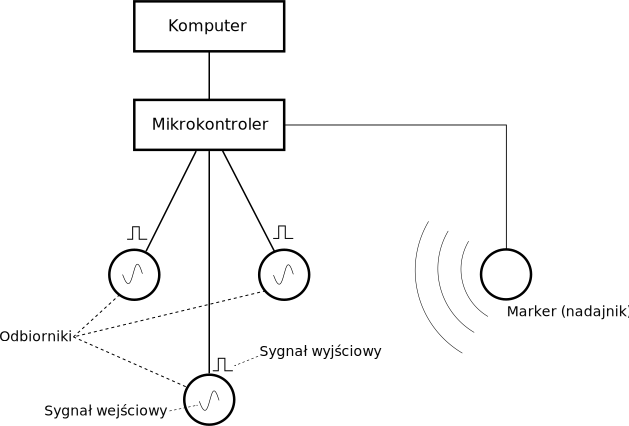
\includegraphics[width=\textwidth]{gfx/diagramy/schemat_blokowy_ukladu}
 \caption{Uproszczony schemat blokowy układu}
 \label{fig:device_scheme}
\end{figure}


\subsubsection{Po dłużce}
Działanie systemu opiera się o fakt, że dźwięk w powietrzu rozchodzi się ze stałą, znaną szybkością.

Ponieważ szybkość ta jest stała, można łatwo wyznaczyć odległość, jaką musiał przebyć dźwięk, aby dotrzeć do odbiornika:

\begin{equation}
 x = v \cdot t
 \label{eq:sound_distance}
\end{equation}
gdzie:\graffito{dodać informację nt. kalibracji - zmiana protokołu na obsługę potwierdzeń, oczekiwanie mikrokontrolera na potwierdzenie, rozpoczynanie kalibracją, wymóg piramidki do kalibracji}
\begin{description}
 \item[$x$] \ppauza~odległość przebyta przez dźwięk,
 \item[$v$] \ppauza~szybkość dźwięku w powietrzu,
 \item[$t$] \ppauza~czas od wysłania sygnału do jego dotarcia do odbiornika. 
\end{description}

Dane, jakie przekazywane są do komputera w celu dalszej obróbki zawierają, poza specyfikacją protokołu, tylko i wyłącznie odczyty z licznika dla każdego z odbiorników.

\paragraph{Przetwarzanie danych}
Aby dane były do czegoś użyteczne, wymagane jest ich przetworzenie. Przetwarzanie danych tej postaci może odbywać się różnorakimi metodami, np.:
\begin{itemize}
 \item rozpoznawanie gestów za pomocą sieci neuronowych,
 \item odtworzenie pozycji markera w trzech wymiarach,
 \item oczekiwanie na przemieszczenie markera do predefiniowanej pozycji,
 \item wiele innych.
\end{itemize}

\paragraph{Odtworzenie pozycji markera}
W celach demonstracyjnych postanowiłem pokazać, jak odtworzyć pozycję markera w trzech wymiarach korzystając tylko z informacji o względnym położeniu odbiorników oraz przekazywanych do komputera danych.
\newline
\newline
Ponieważ odbiorniki znajdują się w różnych, lecz znanych, położeniach w przestrzeni, odległość markera od każdego z nich może być różna.

Aby wyznaczyć położenie markera w trójwymiarowej przestrzeni, mając do dyspozycji odległości od każdego z odbiorników, należy założyć, że odbiorniki są środkami sfer, a promieniem każdej z nich \ppauza odległość, jaką przebył dźwięk od markera do tego odbiornika. Punkt przecięcia się tych sfer będzie pozycją markera.

\begin{figure}
  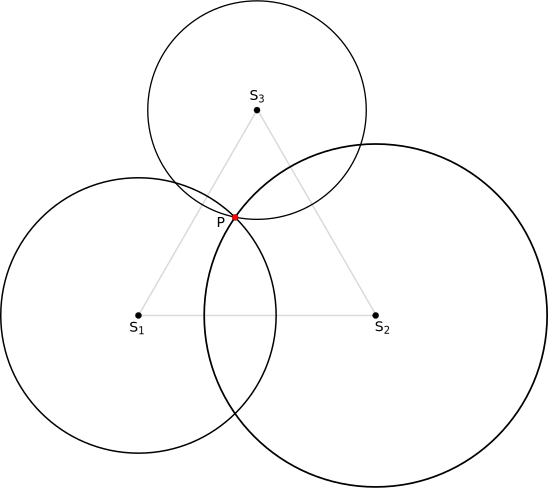
\includegraphics[width=\textwidth]{gfx/diagramy/schemat_przeciecia_sfer}
  \caption{Poglądowy schemat rozmieszczenia czujników}
  \label{fig:schema_spheres}
\end{figure}

Rysunek \ref{fig:schema_spheres}\graffito{W rysunku przyjęto widok ,,od przodu'', tzn. zachodzi $z = 0$ dla wszystkich elementów z wyjątkiem punktu $P$} prezentuje rozmieszczenie odbiorników na płycie testowej. Znajdują się one w punktach oznaczonych odpowiednio jako $S_1$, $S_2$ i $S_3$. Punkt $P$ to punkt przecięcia się sfer.

Ponieważ zastosowano tylko trzy odbiorniki, muszą one leżeć w jednej płaszczyźnie. Powoduje to, że będą istniały dokładnie dwa punkty przecięcia wspomnianych powyżej sfer \ppauza lustrzane do siebie względem płaszczyzny, w której znajdują się odbiorniki.\graffito{dodać notatkę w testach o możliwości wyeliminowania tego 'defektu' poprzez dodanie 4-tego odbiornika, niewspółpłaszczyznowego, jednak spowoduje to wzrost kosztów obliczeń}

Należy wziąć pod uwagę fakt, że zarówno marker jak i odbiorniki są urządzeniami ,,kierunkowymi'', umieszczonymi w tulejach, które powodują, że sygnał nie jest wysyłany dookólnie, lecz w pewnym \ppauza z grubsza określonym \ppauza kierunku, zaś amplituda sygnału odbieranego będzie większa, jeśli będzie on wpadał w tuleję, przez co szansa uznania go za poprawny jest znacznie większa.\graffito{sygnał dochodzący z boku może być ze słaby, aby został wyłapany}

Ta cecha układu została wykorzystana poprzez przeznaczenie układu do noszenia na tułowiu \ppauza łatwo zauważyć, że użytkownikowi ciężko byłoby przesunąć marker zbyt daleko do tyłu, gdyż ograniczałyby go stawy. 

Wykorzystując fakt, że człowiek trzyma ręce w większości przypadków przed sobą, szczególnie jeśli zamierza coś nimi robić, można spokojnie odrzucić jeden z punktów \ppauza ten który znajduje się ,,z tyłu''.

\paragraph{Trilateracja}
Metoda wyznaczenia trójwymiarowej pozycji znając odległości od trzech punktów o znanych współrzędnych nazywana jest \textit{trilateracją}\graffito{dodać info skąd to wiadomo}.

Problem wyznaczenia położenia markera można uprościć, przyjmując określony układ współrzędnych, w którym jeden z odbiorników znajduje się w początku ukłądu współrzędnych, jeden na osi $x$, a trzeci pozostaje ,,swobodny''\graffito{Współrzędna $z$ dla wszsytkich odbiorników równa jest~$0$}. Przyjmując takie rozmieszczenie, które zaprezentowane jest na rysunku \ref{fig:schema_coordinates}, odbiorniki mają współrzędne opdpowiednio:
\begin{matrix}
 $S_1$ & asd
\end{matrix}


\begin{figure}
  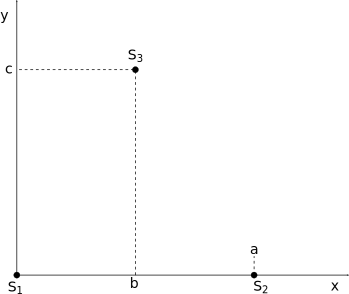
\includegraphics[width=\textwidth]{gfx/diagramy/schemat_uklad_wspolrzednych_clipped}
  \caption{Obrany układ współrzędnych}
  \label{fig:schema_coordinates}
\end{figure}


W celu pomiaru różnicy czasów zdecydowałem się wykorzystać ośmiobitowy timer/counter dostępny w używanym mikrokontrolerze.\graffito{to musi iść gdzieś indziej}

\section{Oprogramowanie}
\subsection{Wykresy}
W celach demonstracji działania stworzyłem program, który pokazuje dane odczytane z urządzenia w dwóch postaciach:
\begin{itemize}
 \item dane odczytane \ppauza rysowany jest wykres danych, jakie zostały wysłane przez urządzenie,
 \item dane przetworzone \ppauza rysowany jest wykres prezentujący pozycję wybranego markera w trzech wymiarach.
\end{itemize}

\myChapter{Implementacja}\label{ch:implementation}
%************************************************

Jako zwolennik wolnego i otwartego oprogramowania starałem się korzystać tylko i wyłącznie z takich właśnie narzędzi.

\graffito{ \includegraphics[width=\marginparwidth]{gfx/gnuhead_inkscape.pdf} Logo Fundacji Wolnego Oprogramowania \ppauza Free Software Foundation \citep{FSF}}Sama praca udostępniana jest na zasadach otwartej licencji \textsc{GNU GPL 3.0}. Wszyzstkie otwarte licencje typu \textsc{GNU GPL} stworzone zostały przez fundację FSF, która też stoi na straży ich przestrzegania.

\section{Oprogramowanie mikrokontrolera}
W pracy wykorzystany został układ \textsc{AVR Atmega8}, będący ośmiobitowym mikrokontrolerem. Sprzęt ten znacznie różni się od architektury znanej z komputerów osobistych \textsmaller{PC} i choć sama idea programowania jest podobna, wszystko pozostawione jest programiście, co w połączeniu z koniecznością programowania na bardzo niskim poziomie, jaki nie jest promowany na studiach, stanowi dodatkowe wyzwanie.

Oprogramowanie zostało stworzone w języku \texttt{C}, wykorzystując do kompilacji kompilator \textsc{avr-gcc} oraz bibliotekę \textsc{avr-libc}, oba udostępniane na zasadach wolnej licencji \textsc{Modified Berkley License}. Do programowania wykorzystałem program \textsc{avrdude} (wolna licencja \textsc{GNU GPL 2} i późniejsze).

\subsection{Wymagania}
Zadaniem tej części oprogramowania jest dostarczenie danych, których obróbką zajmie się komputer. Wymagania, jakie są stawiane to przede wszystkim:
\begin{itemize}
 \item zwięzłość \ppauza program ma robić tylko i wyłącznie to, co absolutnie konieczne, ponieważ wprowadzanie dodatkowego, nadmiarowego kodu będzie powodowało opóźnienia w działaniu, co może przekładać się na
    niestabilność działania,
 \item dokładność \ppauza dostarczanie niepewnych danych mija się z celem pracy, należy więc zadbać o to, aby dane były możliwie najdokładniejsze,
 \item prostota \ppauza ze względu na niewielkie możliwości mikrokontrolera \ppauza w porównaniu do komputerów \ppauza trzeba zoptymalizować wszelkie używane struktury i unikać wykonywania pracy, którą spokojnie może zająć się komputer.
\end{itemize}

Uważam, że program, który napisałem spełnia wszystkie stawiane mu wymagania. Mieści się w niecałych 200 liniach \ppauza nie ma zbędnego kodu, dba o poprawne inicjalizowanie \index{timer}timerów urządzenia \ppauza stara się o dokładność danych, posiada możliwie najmniejsze struktury, które pozwolą przechować dane.

Należy zauważyć, że obrany rozmiar zmiennych, t.j. 8 bitów, został dopasowany do rozmiaru rejestrów mikrokontrolera. W przypadku zmiennych o długości 16 bitów znacznie wzrasta ilość taktów zegara, podczas których dane te są przetwarzane. Krótkie zmienne pozwalają na przechwycenie danych timera \ppauza rejestru \texttt{TCNT0}\graffito{Rejestr \texttt{TCNT0} przechowuje aktualny stan licznika, a zmienna \texttt{ovfCounter} ilość cykli timera.} oraz licznika przepełnień \texttt{ovfCounter} \ppauza w jednym takcie zegara.

Mikrokontroler posiada również drugi, szesnastobitowy timer, którego użycie pozwoliłoby na zwiększenie dokładności, wiązało by się jednak z mankamentem wspomnianym powyżej, zaś precyzja osiągana przez oprogramowanie wykorzystujące timer o wielkości ośmiu bitów, jaka została opisana w sekcji \ref{section:microcontroller_limit}, jest wystarczająca do bardzo dokładnego śledzenia pozycji.

\subsection{Dokładność}\label{section:precision}
\paragraph{Ograniczenia mikrokontrolera}
\label{section:microcontroller_limit}

Dokładność, jaką można uzyskać za pomocą ośmiobitowego timera pracującego w układzie taktowanym zegarem $F_\textrm{cpu} = 8$ MHz wyznacza się w następujący sposób:
\begin{enumerate}
 \item \index{prescaler}prescaler\graffito{Prescaler omówiony zostanie w paragrafie \nameref{sec:prescaler} sekcji \ref{sec:uc_algorithm}.} ustawiony jest na $F_\textrm{cpu}/8$, należy poznać interwał $i$, co jaki wyzwalane będzie przerwanie timera:
    \begin{equation}
      i = \frac{1}{F_\textrm{cpu}/8} = \frac{1}{1~\textrm{MHz}} = 0,000001~\textrm{s} = 0,001~\textrm{ms} = 1~\mu\textrm{s}
      \label{eq:sampling_frequency}
    \end{equation}

 \item znając interwał $i$ oraz szybkość dźwięku w powietrzu $v$, wyznaczyć należy drogę, jaką przebędzie dźwięk w czasie $i$, wykorzystując w tym celu wzór~\ref{eq:sound_distance}:
    \begin{equation}
      x = v \cdot i = 340~\frac{\textrm{m}}{\textrm{s}} \cdot 1~\mu\textrm{s} = 0,34~\textrm{mm}
      \label{eq:microcontroller_limit}
    \end{equation}
\end{enumerate}

Jak pokazuje równanie~\ref{eq:microcontroller_limit}, teoretyczna dokładność sprzętu jest bardzo duża i znacznie przekracza wymagania gier wideo, gdzie w centrum zainteresowania są żwawe, gwałtowne ruchy. Pozwoliłaby ona na prawdopodobne wykorzystanie układu w zastosowaniach wymagających większej precyzji, jak np. modelowanie trójwymiarowe lub wizualizacja danych medycznych.

Ponieważ \index{timer}timer ma tylko osiem bitów, należy spodziewać się, że nastąpi jego przepełnienie zanim zostanie odczytane wzbudzenie pinu. Przepełnienie wystąpi po dokładnie $2^8 = 256$ aktualizacjach timera. Zajmie to $256 \cdot 1~\mu\textrm{s} = 256~\mu\textrm{s}$, a dźwięk w tym czasie zdąży przebyć odległość 
\begin{equation}
 340~\frac{\textrm{m}}{\textrm{s}} \cdot 256~\mu\textrm{s} = 87,04~\textrm{mm}
\end{equation}

Rozdzielczość\graffito{Zmiana ta musiałaby zostać odwzorowana w aplikacjach wykorzystujących ten interfejs sterowania komputerem.} można dalej zwiększyć zmniejszając dzielnik \index{prescaler}prescalera oraz zwiększając częstotliwość pracy mikrokontrolera.

\paragraph{Ograniczenia markerów}
\label{section:sound_limit}
\index{marker}

Ze względu na wykorzystanie nadajników i odbiorników ultradźwiękowych używających dźwięku o częstotliwości $F_{d} = 40$ kHz, należy zbadać jakie narzuca to ograniczenia.

Podobnie jak w przypadku wyliczania ograniczeń mikrokontrolera, tak i w tym przypadku należy wyznaczyć minimalny interwał, w jakim może zajść zmiana.

Za zmianę będziemy przyjmować wzbudzenie pinu mikrokontrolera, co spowodowane jest zaniknięciem nadawanego sygnału. Zdarzenie takie może zajść jedynie co pełny okres fali dźwiękowej. Policzmy więc odległość, jaka będzie dzieliła obraną fazę fali w dwóch ,,sąsiadujących'' okresach:

\begin{enumerate}
 \item wyliczamy okres $T$ fali dźwiękowej:
    \begin{equation}
      T = \frac{1}{F_d} = \frac{1}{40~\textrm{kHz}} = 0,000025~\textrm{s} = 0,025~\textrm{ms} = 25~\mu\textrm{s}
    \end{equation}
 \item znając $T$ skorzystajmy ponownie ze wzoru~\ref{eq:sound_distance}:
    \begin{equation}
      x = v \cdot T = 340~\frac{\textrm{m}}{\textrm{s}} \cdot 25~\mu\textrm{s} = 8,5~\textrm{mm}
      \label{eq:sound_limit}
    \end{equation}
\end{enumerate}

\paragraph{Teoretyczne ograniczenia całego systemu}
Jak pokazują obliczenia przeprowadzone w paragrafach~\nameref{section:microcontroller_limit} i~\nameref{section:sound_limit}, głównym ograniczeniem dokładności bieżącej wersji systemu jest wykorzystanie ,,powolnych'' nadajników i~odbiorników.

Zdecydowałem się na wykorzystanie elementów \graffito{Należy spodziewać się, że czujniki stosowane np. w~aparturze USG są odpowiednio drogie, wykorzystują jednak znacznie wyższe częstotliwości.} o takich właśnie charakterystykach, ponieważ są to jedyne dostępne na rynku, których cena pozwala na ukończenie projektu.

Aby zwiększyć dokładność urządzenia należałoby wymienić nadajniki i odbiorniki na podobne modele, korzystające z wyższych częstotliwości, a także wymienić kwarc generujący częstotliwość dla tych elementów. Bez konieczności przeprogramowywania mikrokontrolera można zastosować elementy używające częstotliwości do
\begin{equation}
 f = \frac{1}{i} = \frac{1}{1~\mu\textrm{s}} = 1~\textrm{MHz}
\end{equation}
gdyż jest to częstotliwość próbkowania określona wzorem \ref{eq:sampling_frequency}.
%\graffito{dodać info o możliwości podkręcenia częstotliwości przez zmniejszenie delay-ów oraz wysyłanie tylko impulsu, zamiast ciągłego sygnału, ponadto używanie w otwrtych przestrzeniach}

\subsection{Algorytm}
\label{sec:uc_algorithm}
Oprogramowanie zapisane w pamięci mikrokontrolera steruje markerami i odbiornikami w następujący sposób:
\begin{enumerate}
 \item \index{prescaler}prescaler urządzenia jest resetowany,\label{enum:prescaler}
 \item uruchamiany jest wewnętrzny licznik urządzenia,
 \item wysyłany jest sygnał, który aktywuje jeden z dwóch markerów, powoduje to rozpoczęcie nadawania sygnału przez ten marker,
 \item następuje aktywne oczekiwanie na ,,wzbudzenie''\graffito{Wzbudzenie pinu to przejście linii z~sygnału niskiego do stanu wysokiego.} pinów wszystkich odbiorników, a czas wzbudzenia każdego z pinów (różnica czasu pomiędzy rozpoczęciem nadawania i odebrania sygnału z~danego odbiornika) jest zapamiętywany,
 \item zatrzymywany jest wewnętrzny timer urządzenia,
 \item dane o odstępach czasowych przekazywane są do komputera,
 \item następuje uśpienie układu, które pozwala na zaniknięcie sygnałów ultradźwiękowych,
 \item cała operacja powtarzana jest dla drugiego markera.
\end{enumerate}
Algorytm ten obrazuje diagram przedstawiony na rysunku \ref{fig:firmware_sequence_diagram}.

\begin{figure}
 % fugly hack
 \hspace{-10em}
 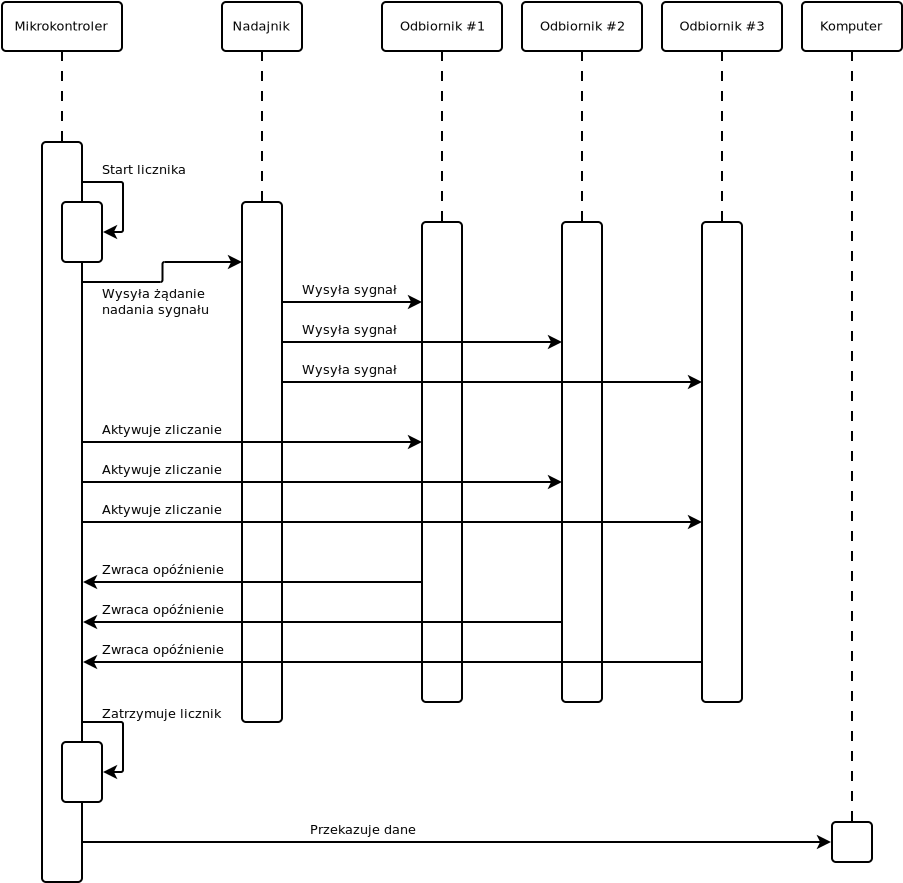
\includegraphics[width=45em]{gfx/diagramy/diagram_sekwencji_sprzetu.pdf}
 \caption{Diagram sekwencji oprogramowania mikrokontrolera}
 \label{fig:firmware_sequence_diagram}
\end{figure}

\paragraph{Prescaler}
\label{sec:prescaler}
W mikrokontroler wbudowany jest \index{prescaler}\textsl{prescaler}, czyli dzielnik częstotliwości, o programowanym stopniu podziału. Jego działanie polega na zliczaniu taktów zegara; gdy wewnętrzny licznik prescalera osiągnie zaprogramowaną wcześniej wartość, wyzwalane jest przerwanie timera oraz następuje przepełnienie licznika, w związku z czym zliczana wartość ,,przekręca się'' i liczenie rozpoczyna się ponownie od zera.

Punkt \ref{enum:prescaler} algorytmu jest bardzo istotny, gdyż nie ma możliwości\graffito{Nawet gdyby możliwość odczytania tej wartości istniała, działanie to wprowadzałoby niepożądane opóźnienia.} sprawdzenia aktualnego stanu licznika prescalera, natomiast rozpoczęcie odliczania może nastąpić w dowolnym momencie czasu, przez co może być niekoniecznie zsynchronizowane z wyzwoleniem przerwania przez prescaler, efektem czego byłyby pomiary, które charakteryzowałyby się pewną zmienną niedokładnością.

\paragraph{Przerwania}
W działaniu programu dużą rolę odgrywają procedury obsługi przerwań (ang. \textsl{ISR \ppauza Interrupt Service Routine}). Są to krótkie fragmenty kodu, które wywoływane są przez mikrokontroler w~momencie zajścia pewnego zdarzenia. Ich użycie pozwala na pewien stopień ,,wielowątkowości'', gdyż (w zależności od ustawienia flag) mogą one przerwać wykonywanie głównego toku programu do momentu, aż przerwania nie zostaną ,,obsłużone'', tzn. instrukcje zawarte w procedurze ISR nie zostaną wykonane.

Implementacja procedur obsługi przerwań jest rozszerzeniem języka C, która jest charakterystyczna dla wybranej rodziny układów i wykorzystanego kompilatora, co powoduje, że wykorzystanie innego kompilatora lub innej rodziny układów wymaga przepisania procedur ISR zgodnie z nowymi wymaganiami.

Jednym z wykorzystanych przerwań jest przerwanie wywoływane przez moduł \texttt{Timer/Counter0}: \texttt{Timer/Counter0 Overflow} (\texttt{TOV0}). Jest ono wyzwalane, gdy licznik \texttt{TCNT0} przekroczy maksymalną możliwą dla niego wartość i rozpocznie się ponowne odliczanie od zera. Zadaniem zawartego w tej procedurze kodu jest tylko i wyłącznie inkrementacja zmiennej \texttt{ovfCounter}, dzięki czemu znana jest ilość przepełnień licznika. W przypadku pominięcia tej danej, pomiary ograniczony byłyby do zaledwie 256 możliwości odległości markera od odbiornika.

Drugie wykorzystane przerwanie jest również przerwaniem licznika i wyzwalane jest przez moduł \texttt{Timer/Counter1}. Jedynym zadaniem tego przerwania jest obsługa jednej z diod, której zadaniem jest wizualne potwierdzenie sprawności i działania układu.

Przykład procedury obsługi przerwania na podstawie opisanej właśnie funkcjonalności prezentuje listing~\ref{lst:interrupt_handler}.

\begin{listing}
  \lstinputlisting[language=C]{listings/atmega_interrupt.c}
  \caption{Procedura obsługi przerwania \texttt{Timer/Counter0 Overflow}}
  \label{lst:interrupt_handler}
\end{listing}

Oznaczenie zmiennej jako \texttt{volatile} oznajmia kompilatorowi, że wszelkie odczyty i zapisy muszą operować na wartości zmiennej z pamięci. W przypadku braku takiego zapisu kompilator podczas kompilowania kodu źródłowego z włączoną flagą optymalizacji może przyjąć, że procedura zmieniająca wartość zmiennej nie jest nigdzie wywoływana, przez co bezpiecznym jest cache-owanie wartości zmiennej, a w efekcie zignoruje skutki wywołania przerwania.

Makro \texttt{ISR(vector [, attributes])} z biblioteki \textsmaller{avr-libc} definiuje następujące po nim ciało funkcji jako procedurę obsługi przerwania. Argument \texttt{vector} jest wymagany i oznacza pozycję w wektorze przerwań mikrokontrolera, do której przypisany ma zostać kod. Argument \texttt{attributes} jest opcjonalny i modyfikuje działanie procedury ISR \ppauza pozwala np. na zagnieżdżanie przerwań, czyli przerwanie przetwarzania procedury ISR przez inne przerwanie.

Wygenerowany wektor przerwań, prezentujący obecność tylko dwóch, wymienionych powyżej, procedur obsługi przerwania prezentuje listing~\ref{lst:interrupt_vector}.

\begin{listing}
  \lstinputlisting{listings/interrupt_vector.txt}
  \caption[Wektor obsługi przerwań]{Wygenerowany wektor obsługi przerwań}
  \label{lst:interrupt_vector}
\end{listing}

Pierwsza pozycja na liście jest punktem wejścia programu, od którego rozpoczyna się wykonywanie kodu. Pozycje z adresów \texttt{0x10} i~\texttt{0x12} to przekierowania do odpowiednio procedur ISR dla przerwań oznaczonych jako \texttt{Timer/Counter0 Overflow} i \texttt{Timer/Counter1 Overflow}.

\section{Oprogramowanie dla komputera}
W celu stworzenia oprogramowania dla komputera wykorzystałem kilka środowisk i bibliotek.

\paragraph{Qt}
Wieloplatformowe środowisko (ang. \textsl{framework}) \textsmaller{Qt}, licencjonowane wolną licencją \textsc{GNU LGPL 2.1} oraz \textsc{GNU GPL 3.0}, składa się z kilku komponentów. W jego skład wchodzą między innymi: biblioteka \textsc{Qt} oraz kompilator \verb|moc|. Wszystkie te elementy znacznie usprawniają pisanie aplikacji w języku \verb|C++| dostarczając metod, które abstrahują od specyfiki wykorzystywanego systemu operacyjnego.

Pisanie nawet skomplikowanych programów z wykorzystaniem \textsc{Qt} jest proste, łatwe, szybkie i przyjemne. Programista świadomy różnic pomiędzy systemami operacyjnymi i delegujący obsługę parametrów do metod dostarczanych przez klasy bibliotek \textsc{Qt} zyskuje możliwość skompilowania swojego kodu pod platformy \textsc{Linux}, \textsc{Windows} oraz \textsc{Mac OS X} bez konieczności jakichkolwiek zmian.

Szerokie spektrum dostarczanych klas (począwszy od kontenerów danych i metod iteracji, przez obsługę urządzeń wejściowych, przez obsługę sieci, aż po rysowanie i zarządzanie grafikami i wiele, wiele innych\ldots) zapewnia, że do zaimplementowania wielu aplikacji nie będzie wymagane wykorzystanie bibliotek trzecich.
\newline
\newline
\textsl{Sygnały i sloty}
Ze względu na intensywne wykorzystywanie w stworzonych aplikacjach połączeń sygnał-slot, zamieszczam poniżej ich opis.

Centralną właściwością środowiska \textsc{Qt}, a jednocześnie jedną z najbardziej odróżniających ten framework od innych, jest mechanizm sygnałów i slotów będący zarządzaną metodą komunikacji pomiędzy obiektami.

Chociaż na pierwszy rzut oka przypomina ona znane dotychczas metody oparte o wywołania zwrotne (ang. \textsl{callback}) i faktycznie się z~nich wywodzi, to jednak różni się od nich w kilku kluczowych aspektach.

Jest to metoda dynamiczna (działająca w runtime). Metoda wywołań zwrotnych wykorzystywana jest głównie do zamodelowania statycznych (tj. znanych już podczas czasu kompilacji - ang. \textsl{compiletime}) powiązań pomiędzy obiektami jak np:
\begin{verse}
użytkownik kliknął przycisk \texttimes~\textrightarrow~wywołaj metodę \texttt{close()}
\end{verse}

W przypadku tym przypisuje się wskaźnik do funkcji do pewnego pola klasy wywołującej, który w momencie zajścia zdarzenia jest wywoływany. Konsekwencją takiego podejścia jest konieczność znania odbiorników w czasie kompilacji, co uniemożliwia np. ładowanie wtyczek w runtime i powiadamiania ich o zdarzeniach w następujący sposób:
\begin{verse}
powiadom wszystkie odbiorniki o zajściu zdarzenia $\omega$
\end{verse}

Zastosowanie w tym miejscu wektorów wskaźników jest jedynie obejściem problemu, a nie jego rozwiązaniem, gdyż nakłada na programistę obowiązek pamiętania o poprawnym przydzielaniu i zwalnianiu pamięci na te elementy, w przypadku aplikacji wielowątkowych szczegółowego analizowania zależności czasowych pomiędzy wywołaniami kodu obiektów, oraz drobiazgowego sprawdzania typów wywołań.

Podejście to wprowadza ponadto nadmiarową i zbędną wiedzę o~odbiornikach do nadajnika.

Rozwiązanie dostarczane przez framework \textsc{Qt} jest elegancką metodą pozbycia się wymienionych wad na rzecz udostępnienia programiście prostego w obsłudze, lecz potężnego i skutecznego, mechanizmu dynamicznego wiązania obiektów w pary nadajnik-odbiornik.

Przekazywane sygnały są ,,wątkowo-bezpieczne'' (ang. \textsl{thread-safe}), co pozwala na przetwarzanie sygnału w innym wątku niż ten, który zainicjował jego wysłanie. Aby zrealizować takie podejście, każdy z~obiektów dziedziczących po klasie \verb|QObject| powinien należeć do jakiegoś wątku, tak aby był on uwzględniany w pętli zdarzeń (ang. \textsl{event loop}), jaka jest przez ten wątek przetwarzana. Domyślnie każdy nowy obiekt przynależy do wątku rodzica, który go utworzył.

Pociąga to za sobą konsekwencję, że jeżeli obiekt nie przynależy do żadnego wątku, to jego zdarzenia nie będą przetwarzane.

W celu uproszczenia obsługi, środowisko \textsc{Qt} domyślnie wykorzystuje do wszystkich obiektów wątek główny aplikacji i jeśli programista jawnie nie usunie z niego obiektów, to ich sygnały będą przetwarzane właśnie w tym wątku.

Aby zintegrować to rozwiązanie z kodem, postanowiono ,,rozszerzyć'' standard\graffito{,,Rozszerzenie'' to wykorzystywane jest tylko i wyłącznie do środowiskia \textsc{Qt}.} języka \verb|C++|. Do istniejących już kwalifikatorów \verb|public|, \verb|private| i~\verb|protected| dodano dwa nowe: \verb|signals| i \verb|slots|.

Kwalifikator \verb|signals| definiuje sygnały. Mają one taką samą strukturę, jak zwykłe metody klasy z następującymi wyjątkami:
\begin{aenumerate}
  \item definicja sygnału jest tylko i wyłącznie jego deklaracją, oznacza to, że sygnał nie posiada żadnego kodu, jest tylko abstrakcyjnym tworem komunikującem zajście pewnego zdarzenia,
  \item sygnały nie mogą zwracać wartości \ppauza zwracanym typem musi być \verb|void|, a wszelkie przekazywane dane zawarte są w argumentach,
  \item sygnały są zawsze publiczne.
\end{aenumerate}

Deklarację pewnej minimalnej klasy zawierającej sygnały prezentuje listing \ref{lst:signals_declaration}.

\begin{listing}
  \lstinputlisting{listings/signals_declaration.cpp}
  \caption{Klasa zawierająca sygnały}
  \label{lst:signals_declaration}
\end{listing}

Jak pokazano, aby klasa mogła wykorzystać mechanizm sygnałów (a także slotów), musi ona dziedziczyć z klasy \verb|QObject| i wywoływać makro \verb|Q_OBJECT| w prywatnej części deklaracji.

Kwalifikator \verb|slots|, jak łatwo się domyślić, deklaruje sloty. Poza dodatkową możliwością wywołania slotu, są to tradycyjne metody klasy i tak samo obowiązują je pozostałe kwalifikatory: \verb|public|, \verb|private| i~\verb|protected|. W odróżnieniu od sygnałów, sloty wymagają dostarczenia implementacji i mogą zwracać wartości.

Deklarację pewnej minimalnej klasy zawierającej sloty prezentuje listing \ref{lst:slots_declaration}.

\begin{listing}
  \lstinputlisting{listings/slots_declaration.cpp}
  \caption{Klasa zawierająca sloty}
  \label{lst:slots_declaration}
\end{listing}

Połączenie emitera ze słuchaczem następuje poprzez wywołanie metody \verb|connect| klasy \verb|QObject|, której argumentami są obiekty nadający i~odbierający, a także nazwy łączonych metod. Sygnatura slotu i sygnału musi być taka sama, z wyjątkiem zwracanego typu.

Użyteczną cechą jest możliwość podłączenia sygnału do sygnału, dzięki czemu zostanie wywołany drugi z sygnałów, a w efekcie podłączone do niego sloty.

Pozostała charakterystyka tego rozwiązania, taka jak przekazywanie meta-typów, rozgraniczenie pomiędzy obiektem nadającym, a odbierającym oraz inne, nie została wykorzystana w stworzonym oprogramowaniu, w związku z czym odsyłam czytelnika do dokumentacji środowiska \textsc{Qt} \citep{Qt}.
\newline
\newline
\textsl{Kompilator moc} Ponieważ powyższe rozwiązanie nie należy do standardu języka \verb|C++|, zaś całe oprogramowanie stworzone przy pomocy środowiska \textsc{Qt} kompilowane jest przy pomocy kompilatora \verb|C++| zgodnego ze standardem ISO/IEC C++\citep{CPPStandard}, takiego jak \texttt{g++}, dostarczany jest wraz z \textsc{Qt} kompilator \texttt{moc}, czyli \textsl{meta-object compiler}.

Zadaniem tego narzędzia jest przeparsowanie dostarczonych plików źródłowych pod kątem odszukania wśród nich deklaracji klas dziedziczących z \verb|QObject|, a zatem wykorzystujących rozszerzone możliwości oferowane przez \textsc{Qt} i wygenerowanie kodu zrozumiałego przez wspomniany wyżej ,,zwykły'' kompilator. Kod dostarczony przez programistę, pozbawiony rozszerzeń \textsc{Qt} oraz kod wygenerowany przez narzędzie \texttt{moc} są kompilowane, a następnie łączone ze sobą na etapie linkowania.

\paragraph{QSerialPort}
Biblioteka \textsc{QSerialPort}, oparta o wolną licencję \textsc{GNU LGPL 2.1}, dostarcza metod komunikacji wykorzystujych port szeregowoy \textsmaller{RS232}. Opiera się ona o środowisko \textsc{Qt}, przez co bardzo łatwo jest zintegrować ją z projektami korzystającymi z tych narzędzi. Podobnie jak samo \textsc{Qt}, biblioteka ta jest wieloplatformowa, co było jednym z~głównych powodów, dla których wybrałem właśnie ją.

Dostarcza ona metody obsługi portów oparte o interfejs \verb|QIODevice| udostępniany przez \textsc{Qt}, które implementowane są z wykorzystaniem natywnych funkcji systemowych dla każdej z platform, dzięki czemu przekazywanie danych odbywa się szybko i sprawnie \citep{QSP}.

\paragraph{Qwt}
Zadaniem tej biblioteki\graffito{\textsc{QWT} oznacza \textsc{Qt Widgets for Technical Applications}.}, opartej o wolną licencję \textsc{Qwt License 1.0} (która z kolei oparta jest o licencję \textsc{GNU LGPL 2.1}), jest rysowanie i~obsługa wykresów. Jest ona, podobnie jak \textsc{QSerialPort}, oparta o środowisko \textsc{Qt}, co zapewnia niedostępny w innym przypadku poziom integracji. Ponieważ poza \textsc{Qt} oraz standardową biblioteką \textsc{libstdc++} nie posiada ona żadnych zewnętrznych zależności, to podobnie jak te projekty jest ona także wieloplatformowa \citep{QWT}.

\paragraph{Bazaar}
\textsc{Bazaar} lub, w skrócie, \textsc{bzr}\graffito{Skrót wziął się od nazwy wykonywanego polecenia \ppauza \texttt{bzr}.}, to dystrybuowany system kontroli wersji, który pozwala na śledzenie i oznaczanie zmian w kodzie źródłowym, dzięki czemu można śledzić rozwój programu, oznaczać wydania, współdzielić kod pomiędzy gałęziami,  przypisywać błędy do rewizji oraz wiele innych. W połączeniu z serwisem \textsc{Launchpad} umożliwia hostowanie kodu w repozytorium on-line oraz wygodne zarządzanie projektem. Oba narzędzia udostępniane są na zasadach wolnych licencji, odpowiednio: \textsc{GNU GPL 2} i późniejsze oraz \textsc{GNU Affero GPL v3} \citep{BZR}.

Całość stworzonej pracy, włączając w to ten dokument, wersjonowane były wykorzystując te narzędzia i należą do projektu nazwanego \texttt{janisozaur-inz} dostępnego pod adresem:
\begin{verse}
  \url{https://launchpad.net/janisozaur-inz}
\end{verse}

\paragraph{Bullet Physics Engine}
Aby uatrakcyjnić prezentację, a zarazem zademonstrować jedno z przykładowych zastosowań systemu, wykorzystałem otwarty silnik fizyki \textsc{Bullet PE}. Jest to dojrzały projekt, wykorzystywany w wielu popularnych grach (np. \textsc{GTA 4}), programach graficznych (\textsc{Blender}), a także na potrzeby produkcji filmowych (\textsc{2012}) \citep{BPE}.

\paragraph{OpenGL}
\textsc{OpenGL} to otwarta biblioteka graficzna, której implementację dostarcza zwykle producent sterowników do posiadanej karty graficznej. Udostępnia ona możliwości tego elementu na potrzeby renderowania, przetwarzania i wyświetlania grafiki trójwymiarowej.

\subsection{Trilaterator}
Pierwsza ze stworzonych aplikacji przeznaczona jest do przeprowadzania trilateracji, o której mowa w sekcji \ref{par:trilateration}. Wykonuje ona automatycznie obliczenia dane wzorami \ref{eq:trilateration_final_x}, \ref{eq:trilateration_final_y} i \ref{eq:trilateration_final_z}. Interfejs aplikacji umożliwia wprowadzanie wszelkich danych dotyczących rozmieszczenia odbiorników jak i markera. Wyniki dokonanych obliczeń prezentowane są w dolnej części programu.

Aplikację wraz z przykładowymi danymi prezentuje rysunek \ref{fig:trilaterator}.

\begin{figure}[t]
 \includegraphics[width=\textwidth]{gfx/trilaterator_triple.png}
 \caption{Trilaterator. Aplikacja dokonująca trilateracji}
 \label{fig:trilaterator}
\end{figure}

Przykładowe dane oraz poprawność zastosowanej metody pokazuje rysunek \ref{fig:trilateration_sample}.

Jak widać, oddalenie odbiorników od siebie na odległość zaledwie kilku centymetrów pozwala badać położenie markera w przestrzeni.

\paragraph{Struktura programu}
Przedstawiony program jest celowo bardzo prosty i sprowadza się tylko do obsługi zdarzenia kliknięcia przycisku, tak aby łatwo można było prześledzić działanie metody. Całą istotę działania programu prezentuje listing~\ref{lst:trilateration}.

\begin{listing}
  \lstinputlisting{listings/trilateration.cpp}
  \caption{Kod dokonujący trilateracji}
  \label{lst:trilateration}
\end{listing}

\paragraph{Dokładność obliczeń}
Należy wziąć pod uwagę fakt, że odległość pomiędzy odbiornikami ma wpływ na wynik obliczeń. Wynika to z operowania przez komputer na danych o skończonej i zmiennej dokładności.

Jeśli marker znajdzie się dostatecznie daleko od odbiorników, może nastąpić spadek precyzji, gdyż dane są reprezentowane w pamięci komputera przez typy zmiennoprzecinkowe i przy małym rozsunięciu odbiorników po wykonaniu działań arytmetycznych, a w szczególności operacji potęgowania i pierwiastkowania, jakie są konieczne do odtworzenia pozycji, utrata precyzji będzie miała znaczący wpływ na wynik obliczeń.

Aby uniknąć tego problemu, odbiorniki \textsl{Nietoperza} rozstawione są na planie trójkąta równobocznego o boku 33cm. Pozwala to na wystarczająco dokładne śledzenie precyzji już za pomocą typu zmiennoprzecinkowego pojedynczej precyzji \verb|float|. Na potrzeby tej demonstracji zdecydowałem się jednak wykorzystać typ \verb|double| dostarczający podwójnej precyzji.

\paragraph{Wieloplatformowość}
Aplikacja ta prezentuje także zalety wykorzystanego środowiska, które może być kompilowane pod wszystkimi trzema znaczącymi systemami operacyjnymi: \textsl{Linux}, \textsl{Windows} oraz \textsl{Mac~OS~X}. Do poprawnego skompilowania nie jest wymagana żadna zmiana kodu.

\begin{figure}
  \includegraphics[width=\textwidth]{gfx/wizualizacja_3d.png}
  \caption{Wizualizacja przykładowych danych}
  \label{fig:trilateration_sample}
\end{figure}

\begin{figure}
 \includegraphics[width=\textwidth]{gfx/uklad_render.png}
 \caption[Model systemu i przyjęty układ współrzędnych]{Model systemu wraz z przyjętym układem współrzędnych. Układ ma swój początek w odbiorniku oznaczonym kolorem żółtym}
 \label{fig:coordinate_system}
\end{figure}

\subsection{Charter}
Kolejna aplikacja prezentująca możliwości systemu służy do rysowania wykresów w czasie rzeczywistym na podstawie danych pobranych z mikrokontrolera. Dla porównania dostępne są dwa rodzaje wykresów jednocześnie:
\begin{itemize}
 \item odległość od odbiornika \ppauza pokazuje odległość wybranego markera od każdego z odbiorników,
 \item położenie \ppauza dokonuje w locie trilateracji dla bieżącej próbki i rysuje wykres położenia wybranego markera w trzech wymiarach, zgodnie z układem odniesienia przedstawionym na rysunku \ref{fig:coordinate_system}.
\end{itemize}

Odległość od odbiorników podawana jest jako wartość licznika odczytana z mikrokontrolera. Aby dokonać konwersji na centymetry, należy (w oparciu o równanie \ref{eq:microcontroller_limit}) przeliczyć:
\begin{equation}
 d = \frac{x \cdot 0,34\textrm{mm}}{10}
\end{equation}
gdzie:
\begin{description}
 \item[$d$] \ppauza~wyznaczona odległość w centymetrach,
 \item[$x$] \ppauza~odległość odczytana z wykresu.
\end{description}

Użytkownik w trakcie działania programu ma możliwość wyboru, którego markera dane powinny być rysowane.

Program dokonuje transformacji układu współrzędnych, aby w efekcie uzyskać układ pokazany na rysunku \ref{fig:coordinate_system}.

Jest to taki sam prawoskrętny układ, jak wykorzystywany w bibliotece \textsc{OpenGL}, co znacząco ułatwia pracę, ponieważ nie jest wymagana żadna dodatkowa konwersja układu współrzędnych aby narysować pozycję markera.

\paragraph{Struktura programu}
Program napisany jest z wykorzystaniem środowiska \textsc{Qt}, ponadto korzysta z bibliotek \textsc{QSerialPort} oraz \textsc{Qwt}.

Po uruchomieniu programu tworzone są obiekty wykresów: instancje klas \verb|PositionPlot| i \verb|DistancePlot|, które dziedziczą z klasy \verb|QwtPlot| i zajmują się rysowaniem odpowiednio wykresów pozycji markera oraz jego odległości, ustawiane są parametry tych obiektów dotyczące skali, legendy oraz uruchamiane są timery odpowiadające za odświeżanie danych. Wykresy przedstawiają dane pobrane w ciągu ostatnich 10 sekund i wraz z przybywaniem kolejnych danych wykres jest przesuwany aby spełnić wymieniony właśnie warunek.

Następuje inicjalizacja pozostałych danych interfejsu użytkownika:
\begin{itemize}
  \item domyślny adres portu szeregowego \ppauza jest to jeden z dwóch fragmentów programu, które zależne są od systemu operacyjnego, gdyż ścieżki do tych plików różnią się pomiędzy sytemami,
  \item wypełniane są dozwolone prędkości komunikacji \ppauza jest to drugi z fragmentów, który zależny jest od systemu,
  \item następuje iteracja przez identyfikatory markerów, które dodawane są do pola umożliwiającego przełączanie pomiędzy markerami.
\end{itemize}

Dane pobierane są od \textsl{Nietoperza} przez obiekt klasy \verb|SamplingThread|, która dziedziczy z klasy \verb|QwtSamplingThread|, będącej implementacją dziedziczonej klasy \verb|QThread|. Klasa \verb|QThread| stanowi niezależny od systemu operacyjnego interfejs do wątku, który jest rozszerzony przez \verb|QwtSamplingThread| o implementację metod pozwalających na okresowe odczytywanie danych. Ponadto klasą bazową dla \verb|QThread| jest \verb|QObject|, dzięki czemu sygnały i sloty dostępne są od razu.

Wątek uruchamiany jest po zakończonym sukcesem otwarciu komunikacji z portem szeregowym wykorzystując w tym celu obiekt klasy \verb|QSerialPort|. W przypadku błędu otwarcia portu emitowany jest sygnał \verb|error(QString)|, który propagowany jest aż do paska stanu \verb|QStatusBar| głównego okna aplikacji celem poinformowania użytkownika, a zainicjowane dane są czyszczone, aby nie dopuścić do wycieku pamięci.

Pomyślnie uruchomiony wątek będzie okresowo, z interwałem określonym w konstruktorze domyślnym
\begin{verbatim}
explicit SamplingThread(QObject *parent = 0);
\end{verbatim}
metodą \verb|setInterval(double)|, sprawdzał nadejście nowych danych.

Klasa \verb|SignalData|, która dziedziczy z klasy \verb|QObject| aby zyskać możliwość wykorzystania slotów i sygnałów, implementuje wzorzec projektowy \verb|singleton|, czyli obiektową metodę zapewnienia dostępności jednej i zawsze tej samej instancji. Uzyskałem to poprzez oznaczenie jedynego dostępnego konstruktora kwalifikatorem \verb|private| i zaimplementowałem statyczną metodę zwracającą referencję do statycznej zmiennej tworzonej w tej metodzie:
\begin{verbatimtab}
class SignalData : public QObject
{
	Q_OBJECT
	SignalData();
public:
	static SignalData &instance();
\end{verbatimtab}

Instancja ta tworzona jest dopiero podczas pierwszego wywołania metody \verb|instance()| i ,,żyje'' aż do końca działania aplikacji. Konstruktor tej klasy dokonuje iteracji przez dostępne markery i inicjalizuje lokalne bufory danych dla każdego z markerów. Aby uniknąć konieczności deklarowania pola dla każdego z markerów, co wykluczyłoby prezentowaną poniżej metodę rozszerzania o kolejne markery, zastosowałem kontener \verb|QHash|, którego kluczem jest identyfikator markera \verb|Sample::Marker|, zaś wartością tablica \verb|QVector| zawierająca dane próbek. Analogiczne rozwiązanie zaimplementowałem dla wykorzystywanych przez \textsc{QWT} prostokątów otaczających, lecz w tym przypadku wartością kontenera jest klasa \verb|QRectF| opisująca prostokąt za pomocą danych zmiennoprzecinkowych.

Celem tej klasy jest zapewnienie interfejsu do buforowania i rozdysponowywania danych, który abstrahuje od implementacji metody faktycznie pobierającej dane.

Po odczytaniu danych z portu szeregowego dopisywane są one do dynamicznej tablicy będącej polem \verb|SamplingThread|. Dopiero teraz następuje synchronizacja i identyfikacja raportów, zgodnie z algorytmem \ref{alg:sync} (str. \pageref{alg:sync}).

Jeśli udało się zsynchronizować dane, co oznacza, że przybyła przynajmniej jedna próbka, emitowany jest sygnał \verb|dataArrived()|, którego odbiorcą jest metoda \verb|SignalData::fetchSamples()|. Pobiera ona dane z \verb|SamplingThread| i dla każdej nowej próbki dopisuje ją do lokalnego bufora, a także przetwarza aktualizując na tej podstawie prostokąt otaczający.

Ponieważ pobranie próbek w metodzie \verb|SamplingThread::append()| oraz ich zbuforowanie w metodzie \verb|SignalData::fetchSamples()| na potrzeby \textsc{QWT} ma miejsce w różnych wątkach, zadbałem o poprawną synchronizację tych zdarzeń w czasie \ppauza niedopuszczalnym jest przekazywanie danych (które usuwa informację pierwotną) podczas dopisywania nowych danych. Serializacji tych wywołań dokonałem wykorzystując obiekt klasy \verb|QMutex|, który blokowany jest przed rozpoczęciem operacji na krytycznych danych i zwalniany po ich przetworzeniu.

Z pomocą przychodzi tutaj klasa \verb|QMutexLocker|, która w swoim konstruktorze, przyjmującym jako argument tylko wskaźnik do obiektu \verb|QMutex|, blokuje mutex, zaś destruktor odblokowuje go. Dzięki temu, tworząc automatyczną zmienną na początku każdej metody operującej na krytycznych danych zapewniam, że dostęp do nich jest ekskluzywny, tzn. w dowolnym momencie dane te przetwarzane są przez maksymalnie jeden wątek.

Klasy wykresów są okresowo wzbudzane przez timer, którego interwał z jednej strony zsynchronizowany jest z pojawianiem się nowych próbek, natomiast z drugiej działa odrobinę wolniej, aby oszczędzać czas procesora wymagany na odrysowanie nowych danych. Pomimo tego wykres przesuwany jest płynnie.

Biblioteka \textsc{QWT} pozwala na buforowanie rysowanych wykresów, dzięki czemu wywołanie slotu \verb|replot()| wykresu spowoduje narysowanie tylko nowych punktów, co znacznie oszczędza czas procesora.

W pierwszym podejściu do implementacji przesuwania wykresu wykorzystałem zmianę skali osi X przesuwając wyświetlany fragment zgodnie z nadchodzącymi danymi. Okazało się to problematyczne, gdyż jak wspomina autor wykorzystanej biblioteki (\citep{UweRathmannNewsgroup}), po zmianie osi wymagane jest odrysowanie całego wykresu.

Aby ominąć ten defekt wykorzystałem klasę \verb|QwtPlotPanner| która przesuwa widoczny zakres wykresu nie powodując przy tym unieważnienia bufora. Natknąłem się jednak tutaj na problem, gdyż slot dokonujący przesunięcia oznaczony był jako prywatny. Ratunkiem okazała się możliwość podpięcia sygnału do sygnału \ppauza emitując swój sygnał wyzwalałem istniejący sygnał tej klasy do wywołania prywatnej metody, której efektem było przesunięcie widocznego fragmentu wykresu. W efekcie użycie procesora znacznie spadło.

\paragraph{Rozszerzanie obsługi o dodatkowe markery}
Chociaż dostępna aktualnie wersja sprzętu zaprojektowana jest do obsługi tylko i~wyłącznie dwóch markerów, to prezentowany program przygotowany został w sposób pozwalający na obsługę dowolnej ilości markerów.

Zadbałem o to, aby dodawanie markerów było możliwie proste dla programisty. Wykorzystałem w tym celu mało znaną możliwość, jaką oferuje środowisko \textsc{Qt}, tj. jawne wykorzystanie meta-obiektów.

Deklarując próbkę jako klasę \verb|Sample|, która dziedziczy z podstawowej klasy środowiska \textsc{Qt}, \verb|QObject|, możliwe jest pozyskanie w czasie działania programu (ang. \textsl{runtime}) dostępu do pewnych danych, które w innym przypadku byłyby niedostępne lub dostęp do nich wymagałby od programisty dużej gimnastyki, a nawet wykorzystania bibliotek trzecich takich jak np. \textsc{Boost}.

Podejście takie wymusiło na mnie jednak dostarczenie publicznych implementacji konstruktora domyślnego, konstruktora kopiującego oraz operatora przypisania:
\begin{verbatimtab}
public:
	Sample(QObject *parent = 0);
	Sample(const Sample &other);
	Sample &operator =(const Sample &other);
\end{verbatimtab}
gdyż w klasie \verb|QObject| są to metody prywatne, co uniemożliwia wykorzystywane w kodzie programu kopiowanie i tworzenie automatycznych zmiennych tego typu.

Jedną z możliwości środowiska \textsc{Qt} jest zarejestrowanie danego typu wyliczeniowego \verb|enum| w systemie meta-obiektów poprzez wywołanie makra \verb|Q_ENUMS|:
\begin{verbatimtab}
class Sample : public QObject
{
	Q_OBJECT;
	Q_ENUMS(Marker);
public:
	enum Marker {Blue = 1, Yellow = 2};
	(...)
\end{verbatimtab}

Działanie to pozwala na dostęp do tego typu \verb|enum| w działającym programie za pomocą meta-właściwości. Możliwe jest nie tylko poznanie zarejestrowanych w klasie typów wyliczeniowych, ale także iteracja przez zarówno klucze, jak i właściwości.

Wykorzystanie tej cechy powoduje, że do dodania dodatkowego markera jedyne wymagania, jakich spełnienie musi zapewnić programista to:
\begin{aenumerate}
  \item dodanie identyfikatora markera do typu \verb|Sample::Marker|,
  \item poprawienie kodu wątku obsługującego odczytywanie danych, aby obsłużył zmodyfikowany protokół.\label{item:modify_protocol}
\end{aenumerate}

Jeśli protokół nie zostanie zmieniony, to punkt \ref{item:modify_protocol} nie jest wymagany.

Jak widać dodanie nowego markera jest zadaniem trywialnym.

Chociaż kosztem łatwości rozszerzalności oprogramowania wymaganych jest kilka wywołań funkcji więcej, to nie ma to znaczącego wpływu na wydajność programu.

Program, podczas przykładowego uruchomienia, zaprezentowany jest na rysunku \ref{fig:charter}.

\begin{figure}
  \includegraphics[width=\textwidth]{gfx/charter.png}
  \caption{Program \textsl{Charter} w działaniu}
  \label{fig:charter}
\end{figure}


\subsection{Stickman}
\label{sec:app_stickman}
Trzecią i ostatnią, a zarazem najciekawszą, z punktu widzenia użytkownika końcowego, stworzoną aplikacją demo jest \textsl{Stickman}.

Zadaniem tej aplikacji jest odwzorowywanie ruchów użytkownika na ekranie komputera. W głównej części aplikacji rysowana jest figurka imitująca użytkownika, której ruchy rąk odpowiadają ruchom wykonywanym przez użytkownika.

Dzięki zastosowaniu silnika fizyki możliwa jest prezentacja interakcji z wirtualnym otoczeniem, jaka możliwa jest poprzez śledzenie ruchów.

Aplikację prezentuje rysunek \ref{fig:stickman}.

\begin{sidewaysfigure}
  \includegraphics[width=\textwidth]{gfx/stickman.png}
  \caption[Stickman]{Stickman. Wirtualna postać siejąca postrach wśród kolorowych pudełek}
  \label{fig:stickman}
\end{sidewaysfigure}


\paragraph{Kalibracja}
Ze względu na możliwość wykorzystania \textsl{Nietoperza} przez różnych użytkowników, do poprawnego działania tej aplikacji wymagane jest przeprowadzenie kalibracji, która dostosowywuje parametry aplikacji do aktualnego użytkownika.

Stworzyłem dwie metody kalibracji:
\begin{itemize}
  \item zwykła,
  \item eksperymentalna.
\end{itemize}

\noindent\textsl{Kalibracja zwykła} W trybie zwykłym możliwe jest przystosowanie systemu do działania podczas noszenia przez użytkownika. Jest to prostsza z dwóch metod, która wykorzystuje zmiany pozycji względem oczekiwanych osi do odwzorowania ruchów rękoma. Do przeprowadzenia tej kalibracji potrzebne jest pobranie dwóch punktów kontrolnych:
\begin{itemize}
  \item punkt bliski, czyli taki, który znajduje się przy ramieniu użytkownika,
  \item punkt daleki, czyli taki, który znajduje się na w miejscu, w którym będzie ręka użytkownika gdy zostanie ona wyprostowana przed siebie.
\end{itemize}

Na podstawie tych informacji można wyznaczyć długość ręki (długość wektora pomiędzy tymi punktami), przesunięcie ramienia względem początku układu współrzędnych oraz ,,domyślne'' wychylenie ręki w płaszczyznach XZ (poziome) oraz YZ (pionowe).

Każda kolejna pozyskana próbka posłuży do sprawdzenia względnej pozycji wobec punktu bliskiego i dalekiego, a następnie na podstawie odwrotnych równań trygonometrycznych wyznaczone zostaną kąty, o jakie należało będzie obrócić rękę wokół osi X oraz Y.

Rysowana figurka potrafi także, na podstawie długości wektora mającego początek w punkcie bliskim, zaś koniec w aktualnej próbce, zginać rękę. Działanie to jest jednak ograniczone do tylko i wyłącznie jednej płaszczyzny, ponieważ nie przewidziano pozyskania informacji dotyczącej pozycji łokcia. Może zatem istnieć wiele takich ustawień ręki, które spowodują przesunięcie markera do tej samej pozycji, lecz dla aplikacji tej wszystkie one będą jednakowe.
\newline
\newline
\textsl{Kalibracja eksperymentalna} Drugi typ kalibracji, znacznie bardziej złożony od pierwszego, w założeniu pozwalać miał na wykorzystanie \textsl{Nietoperza} z dowolnej pozycji. Pozostało to niestety tylko założeniem, gdyż pomimo mnogich testów i rozważań teoretycznych nie udało się doprowadzić tej metody do stanu pełnej sprawności \ppauza chociaż wielokrotnie wydawało się, że wszystko już działa, to kolejny test pokazywał, że byłem w błędzie.

Do przeprowadzenia tej metody kalibracji wymagana jest znajomość położenia jednego punktu więcej niż ma to miejsce przy kalibracji metodą zwykłą. Wynika to z konieczności ponownego ustawienia trójwymiarowego układu współrzędnych, a znając tylko dwa punkty, wiadomo, że są one współliniowe, zaś dookoła prostej możliwy jest dowolny obrót. Trzeci, niewspółliniowy, punkt pozwoli na określenie dokładnej translacji i rotacji.

Odwracając tę transformację, tzn. znajdując takie przekształcenie, które zmieni pozyskany z próbek układ współrzędnych na układ jaki prezentowany jest na rysunku \ref{fig:coordinate_system}, możliwe byłoby dokonywanie normalizacji pozostałych próbek za pomocą tej samej transformacji. Pozwoliłoby to na wykorzystanie metody analogicznej jak w przypadku kalibracji zwykłej.

\paragraph{Struktura programu}
Program oparty został o istniejące wcześniej źródła programu \textsmaller{Charter}. Głównym współdzielonym fragmentem jest klasa \verb|SignalData| oraz kod wątku dokonującego odbierania danych z portu szeregowego (klasa \verb|SamplingThread|). Nie jest to jednak dokładna kopia, gdyż w tym przypadku nie istnieje potrzeba zapewnienia rozszerzalności o nowe markery (człowiek ma tylko dwie ręce, a dodanie śledzenia innych kończyn wymagałoby dopisania ich faktycznej obsługi \ppauza w odróżnieniu od wykresów, gdzie dane dla każdego z~markerów są takiej samej struktury). Ponadto program ten nie wykorzystuje biblioteki \textsc{QWT}, wymagane w związku z tym było dostarczenie własnej implementacji pętli zdarzeń.

Wspomniana pętla zdarzeń, która stanowi ciało wirtualnej metody \verb|run()|, to prosta pętla \verb|while|, która usypiana jest na zadany interwał, po czym wywołuje funkcję odpytującą port o nowe dane. Aby móc poprawnie zakończyć działanie wątku, w każdej iteracji sprawdzany jest stan zmiennej \verb|mRun|, która określa, czy wątek ma wciąż działać \ppauza ma ona wtedy wartość \verb|true|. Podczas zamykania programu usuwany jest obiekt tego wątku, a jego destruktor wywołuje metodę \verb|stop()|, która zapewnia bezpieczny sposób zwolnienia zasobów i pozamykania otwartych połączeń.

Klasa \verb|GLWidget| odpowiada za wyświetlanie sceny za pomocą biblioteki \textsc{OpenGL}. Osadzone są w niej również instancje obiektów odpowiedzialnych za przetwarzanie zdarzeń fizycznych. Akcje te są od siebie niezależne i możliwa jest sytuacja, gdy nastąpi wyświetlenie kilku klatek z takim samym ustawieniem elementów z powodu nieprzetworzenia danych świata fizycznego pomiędzy nimi, jak i sytuacja odwrotna, czyli pominięcie wyświetlenia pewnych danych dostarczonych przez silnik fizyki.

Separacja tych zdarzeń ma na celu umożliwienie przetwarzania danych w sposób niezależny, gdyż nie jest możliwym przewidzenie, jak dużo czasu zajmie wyrenderowanie i wyświetlenie klatki oraz obliczenie nowych pozycji ciał przez silnik fizyki. Nominalnie odświeżanie klatek następuje co 20ms, zaś krok symulacji silnika fizyki wywoływany jest co 15ms.

Przybycie każdego raportu powoduje aktualizację stanu pól klasy \verb|GLWidget| oraz ponowne przeliczenie kątów w zgięciach ręki. W miejscu dłoni każdej z rąk umocowana jest sfera, która jest ciałem kinematycznym\graffito{Ciało kinematyczne może powodować akcje w silniku fizyki, lecz nie jest ich odbiorcą.}. Pozwala to na uderzenie ustawionych pudełek i obserwację ich zachowań.

Możliwe jest włączanie i wyłączanie rysowania wybarnych komponentów sceny w trakcie działania programu, co pozwala na dokładniejszą analizę jego działania.

Ponieważ elementy interfejsu zajmują znaczną część ekranu, nie pozostawiając wiele na obszar renderowania, zgrupowałem je w karty, które dodatkowo można ukryć, pozostawiając na ekranie miejsce tylko na wyrenderowany obraz. Przywracanie paska opcji odbywa się z poziomu menu programu.

Program umożliwia też przeprowadzenie prostego testu wydajności: procedura przekształcania układu współrzędnych w trybie kalibracji eksperymentalnej wywoływana jest 100000 razy, a sumaryczny czas, jaki zajęło to działanie wypisywany jest na standardowym wyjściu błędów \verb|stderr|.

\section{Protokół}
\label{sec:protocol}
\index{protokół}
Mikrokontroler komunikuje się z komputerem za pomocą standardu \index{RS232}\textsmaller{RS232}, do obsługi którego wykorzystuje moduł \index{USART}\textsmaller{USART}. Aby uzgodnić dane pomiędzy komputerem a mikrokontrolerem, zaprojektowałem protokół, zgodnie z którym następuje przekazanie danych.

Protokół taki powinien zawierać możliwie mało nadmiarowych danych, umożliwiać synchronizację bez względu na moment włączenia nadajnika (mikrokontrolera) względem odbiornika (komputera) oraz zawierać wszystkie potrzebne informacje do odtworzenia położenia wszystkich obsługiwanych markerów.

Mianem \index{raport}\emph{raportu} będziemy nazywać jeden pełen zestaw danych, jakie przesyła do komputera mikrokontroler.

Raport w zaprojektowanym protokole prezentuje rysunek \ref{fig:protocol}.

\begin{figure}
 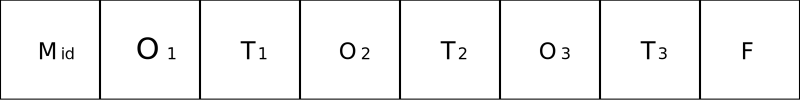
\includegraphics[width=\textwidth]{gfx/diagramy/protokol.pdf}
 \caption[Schemat raportu]{Raport w protokole komunikacji mikrokontrolera z komputerem}
 \label{fig:protocol}
\end{figure}

Każda ramka składa się z ośmiu bajtów, do których należą:
\begin{itemize}
 \item \texttt{M$_\textrm{\texttt{id}}$} \ppauza $id$ markera,
 \item \texttt{O$_n$} \ppauza wartość zmiennej \texttt{ovfCounter} w chwili wzbudzenia pinu odbiornika $n$,
 \item \texttt{T$_n$} \ppauza wartość rejestru \texttt{TCNT0} w chwili wzbudzenia pinu odbiornika $n$,
 \item \texttt{F} \ppauza zawsze \texttt{0xFF}.
\end{itemize}

Pole \texttt{F} wraz z polem \texttt{M$_\textrm{\texttt{id}}$} służy do synchronizacji danych odbieranych przez komputer. Metodę \index{synchronizacja}synchronizacji prezentuje algorytm \ref{alg:sync}.

\begin{algorithm}
\caption{Metoda synchronizacji danych}
\label{alg:sync}
\begin{algorithmic}[1]
  \REQUIRE \texttt{dane} \ppauza tablica dynamiczna, do której końca dopisywane są przychodzące dane
  \WHILE{\texttt{dane.count() $\geq$ 8}}
    \WHILE{\texttt{dane.count() $\geq$ 8 \&\& (dane[0] != M$_\textrm{\texttt{id}}$ \textbar{}\textbar{} dane[7] != 0x77})}
      \STATE usuń(\texttt{dane[0]})
    \ENDWHILE
  \ENDWHILE
\end{algorithmic}
\end{algorithm}

Należy zauważyć, że poza samymi danym protokołu, pomiędzy kompterem, a mikrokontrolerem przekazywane są również dane kontrolne standardu \index{RS232}RS232:
\begin{itemize}
  \item bity startu,
  \item bity stopu.
\end{itemize}

Zrezygnowałem natomiast z funkcji:
\begin{itemize}
 \item bity parzystości \ppauza te dane kontrolne bardzo słabo spełniają swoją rolę, gdyż są bardzo podatne na zakłócenia, które powodują przestawienie parzystej ilości bitów,
 \item kontrola przepływu \ppauza funkcjonalność nie jest dostępna w mikrokontrolerze.
 \item więcej niż 8 bitów w jednej ramce \ppauza chociaż mikrokontroler oferuje przesłanie do 9 bitów danych w jednej ramce, to wykorzystanie tej funkcjonalności znacznie ograniczyłoby funkcjonalność platformy ze względu na fakt, iż układy stosowane w komputerach rzadko kiedy oferują obsługę takich ramek\graffito{Obsługa 9-bitowych ramek wymaga też specjalnego oprogramowania.}, ponadto spowodowałoby dodatkowy narzut pracy na mikrokontrolerze związany z podziałem danych na 9-bitowe części, nie oferując przy tym żadnego wzrostu wydajności \ppauza przesłanie 64 bitów (8 bajtów) wymagałoby i tak 8 ramek.
\end{itemize}

Pełna ramka standardu RS232 składa się zatem z 10 bitów:
\begin{enumerate}
 \item bit startu,
 \item 8 bitów danych,
 \item bit stopu.
\end{enumerate}

Protokół w jego pełnej okazałości demonstruje rysunek \ref{fig:cutecom}.

\begin{figure}
  \includegraphics[width=327px]{gfx/cutecom.png}
  \caption{Cutecom \ppauza aplikacja ukazująca ruch na porcie szeregowym wykorzystując opisywany protokół}
  \label{fig:cutecom}
\end{figure}

\myChapter{Testy}\label{ch:tests}
%************************************************

\section{Cele}

Głównym zadaniem przeprowadzonych testów było zbadanie zachowania stworzonego systemu i oprogramowania pod kątem wykorzystania w grach wideo\graffito{Wynika to ze studiowania na specjalności Technologii Gier i Symulacji Komputerowych}. Nie jest jednak trudno sobie wyobrazić inne dziedziny, w których można wykorzystać systemu, jak np.:
\begin{itemize}
 \item medycyna \ppauza manipulacja trójwymiarowymi obrazami skanów pacjentów,
 \item cyfrowe modelarstwo \ppauza szybkie prototypowanie modeli,
 \item tworzenie filmów \ppauza przechwytywanie ruchu.
\end{itemize}

Głównym atutem systemu w tych dziedzinach jest naturalny sposób manipulacji i~interakcji z komputerem ze względu na pobieranie dodatkowo \ppauza w odróżnieniu od standardowego zostawu klawiatura + myszka \ppauza trzeciego wymiaru.

\section{Metody}
Aby określić przydatność systemu, należy zbadać kilka czynników. Ich wagi będą różnić się, w zależności od planowanego wykorzystania, jednak można zauważyć, że należy dążyć do optymalizacji cech takich jak:
\begin{itemize}
 \item dokładność,
 \item stabilność,
 \item niezawodność,
 \item prostota użytkowania,
 \item kompatybliność z oprogramowaniem,
 \item szybkość.
\end{itemize}


\section{Wyniki}
% dokladnosc
\paragraph{Dokładność}
Dokładność systemu została już określona w sekcji \ref{section:precision}, pozwolę więc sobie jedynie przytoczyć obliczone parametry.

Istnieją dwa rodzaje ograniczeń: spowodowane stworzonym oprogramowaniem oraz spowodowane wykorzystanym sprzętem. Ominięcie tych pierwszych jest stosunkowo łatwe\graffito{Trzeba liczyć się z faktem, że można natknąć się na ograniczenia mikrokontrolera} i~wymaga tylko zmiany pewnych parametrów oraz ponowne zaprogramowanie układu. W przypadku drugiego typu ograniczeń należy spodziewać się konieczności modyfikacji układu, jeśli chciałoby się zwiększać dokładność.

Mikrokontroler jest w stanie mierzyć pozycję markera z dokładnością do 0,34mm\graffito{Równania odpowiednio \ref{eq:microcontroller_limit} i \ref{eq:sound_limit}}, natomiast wykorzystanie sygnałów ultradźwiękowych o częstotliowści 40kHz nakłada na system ograniczenie dokładności do 8,5mm, a zatem ograniczenie całego systemu wynosi 8,5mm.

Chociaż w wielu przypadkach taka dokładność jest zupełnie wystarczająca, pozostawia jednak trochę do życzenia.

% stabilnosc
\paragraph{Stabilność}
Pomimo przytoczonej powyżej, relatywnie małej, dokładności układ wykazuje pewną niestabilność, która objawia się drganiem odtworzonej pozycji markera. Widać to dobrze na rysunku \ref{fig:charter_shaky}, którego górna część pokazuje odtworzoną pozycję w trzech wymiarach. Wszystkie dane, a w szczególności wartość $Y$, wykazują kilkucentymetrowe drgania pomimo stabilnego umocowania zarówno układu jak i markera.

\begin{figure}
 \includegraphics[width=\textwidth]{gfx/charter_shaky.png}
 \caption[Wykres pozycji i odległości jednego z markerów]{Wykres pozycji i odległości od czujników jednego z~markerów w~stałej pozycji}
 \label{fig:charter_shaky}
\end{figure}

% niezawodność
\graffito{coś trzeba napisać o niezawodności}

% prostota użytkowania
\paragraph{Prostota użytkowania}
Starałem się zaprojektować system w taki sposób, aby korzystanie z niego było możliwie proste, jednak wymogi systemu powodują, że korzystanie z niego nie jest tak proste, jak ma to miejsce w przypadku systemów ,,konkurencyjnych'' \graffito{Wiimote, Sixaxis, Kinect...}.

Aby móc w pełni wykorzystać oprogramowanie, a~w~szczególności program \textsmaller{Viewer}\graffito{ponazywać programy}, wymagane jest dokonanie \index{kalibracja}kalibracji. Nie jest to czynność trudna, lecz wymóg wykonania jej każdorazowo po uruchomieniu może zniechęcać użytkowników.

Kalibracja ma na celu ustawienie wewnętrznych parametrów programu, które będą pozwalały na dokładniejsze odwzorowanie ruchów użytkownika. Na wykorzystywane parametry składają się długość ręki, pozycja ramienia i rotacja ramienia.

W zależności od trybu kalibracji wymagane jest pobranie dwóch lub trzech punktów kontrolnych; w tym celu należy:
\begin{enumerate}
 \item jeśli została już dokonana kalibracja od uruchomienia programu, należy ją zresetować za pomocą stosownego przycisku,
 \item ustawić rękę (marker) w ustalonej pozycji względem ciała,
 \item nacisnąć przycisk informujący program o ustawieniu markera,
 \item powtórzyć czynność dla pozostałych punktów kontrolnych,
 \item gdy zostaną pobrane wszystkie punkty kontrolne, należy nacisnąć przycisk wyzwalający kalibrację, co spowoduje ustawienie trybu skalibrowanego.
\end{enumerate}

Wykonanie tej procedury spowoduje przekształcanie układu współrzędnych urządzenia na układ współrzędnych związany z użytkownikiem.

% kompatybilność z oprogramowaniem
\paragraph{Kompatybilność z oprogramowaniem}
Program wykorzystuje do komunikacji z komputerem protokół \index{RS232}\textsmaller{RS232}. Jest to standard komunikacji szeregowej niegdyś bardzo często dostępny w komputerach, jednak dziś odpowiednie złącza i interfejsy dostępne są za sprawą stosunkowo niedrogich adapterów wpinanych do portu \index{USB}\textsmaller{USB}.

Chociaż do uruchomienia komunikacji z wykorzystaniem modułu \index{USART}\textsmaller{USART}\graffito{\textsmaller{USART} \ppauza Universal Synchronous and Asynchronous serial Receiver and Transmitter} mikrokontrolera nie jest wymagane stosowanie zewnętrznego oscylatora, to jego wykorzystanie zmniejsza ilość błędów, jakie mogą zachodzić podczas transmisji.

Ze względu na brak możliwości zakupu stosownego oscylatora, zdecydowałem się wykorzystać wbudowany w mikrokontroler zadajnik częstotliowści. W takiej konfiguracji, w przypadku transmisji danych z prędkością 9600bps\graffito{\index{bps}bps \ppauza baud per second; symbole na sekundę; w~przypadku RS232 1 symbol to 1 bit} błąd wynosi zaledwie 0,2\%.\label{sec:usart_error}\graffito{dopisać tłumaczenie dlaczego tak jest}

Moje doświadczenie z mikrokontrolerami pokazuje, że wartość ta jest dostatecznie mała, aby można było założyć, że trasmisja jest dokładna.

Wykorzystany do komunikacji interfejs oraz zaproponowany protokół\graffito{Protokół opisano w~sekcji \ref{sec:protocol}} jest bardzo prosty, co pozwala na dodanie obsługi systemu do dowolnego programu pragnącego skorzystać z tej możliwości znikomym nakładem pracy.

Stanowiłoby to duży atut systemu w przypadku jego popularyzacji.

\paragraph{Szybkość}
Niestety, szybkość układu pozostawia wiele do życzenia.

Istnieje kilka czynników, które można podejrzewać o spowalnianie działania. Rozpatrzmy po kolei każdy z nich.

\textsl{Wydajność obliczeń}\graffito{Obliczenia dotyczą głównie przekształcania układu współrzędnych} \ppauza aby nie obciążać zbędną pracą mikrokontrolera, który na dodatek nie posiada wystarczającej mocy obliczeniowej, obliczenia dokonywane są dopiero na komputerze\graffito{Jeśli dana aplikacja faktycznie takich obliczeń wymaga}. Chociaż w celu pełnego przywrócenia układu współrzędnych użytkownika z dowolnego ustawienia odbiorników wymaganych jest kilka obrotów oraz translacji punktów\graffito{Obrót i translacja wymagają mnożenia macierzy 4\texttimes 4 przez trójwymiarowy wektor}, a także obliczanie wartości odwrotnych funkcji trygonometrycznych oraz normalizacje trójwymiarowych wektorów, to wykorzystanie procesora przez aplikację zarówno na laptopie wyposażonym w procesor \textsmaller{Intel Core 2 Duo T7700 2,40GHz} oraz komputerze stacjonarnym z procesorerm \textsmaller{Intel Core 2 Duo E6420 2,13GHz} jest znikome.

Przeprowadzone testy pokazują, że wspomniany powyżej laptop wykonuje 100000 pełnych cykli takich obliczeń w przeciągu 448ms, co oznacza, że jeden cykl obliczeń zajmuje niecałe 5\textmu s.

% Przyjmuję więc, że praca ta wykonywana jest na tyle szybko, żeby nie spowalniała działania całego systemu\graffito{dodać testy wydajności - ilość pełnych transformacji układu na sekundę}.

\textsl{Szybkość transmisji danych}
Szybkość transmisji danych zależy głównie od ilości danych przesyłanych protokołem określonym w sekcji \ref{sec:protocol} oraz prędkości tego protokołu.

W związku z błędami omówionymi w sekcji \ref{sec:usart_error}, możliwe są dwie prędkości, w których stopień błędu wynosi 2\textperthousand:
\begin{itemize}
 \item 9600bps
 \item 38400bps
\end{itemize}

Czas przesłania jednego raportu obliczamy wzorem:
\begin{equation}
 t = \frac{c \cdot r}{s} \cdot 1000
\end{equation}
gdzie:
\begin{description}
 \item[$t$] \ppauza~czas potrzebny na przesłanie raportu liczony w milisekundach,
 \item[$c$] \ppauza~ilość bitów w ramce, dla wykorzystanego trybu standardu \index{RS232}RS232 jest to wartość stała $c = 10$,
 \item[$r$] \ppauza~ilość bajtów w raporcie, dla zaprojektowanego protokołu jest to wartość stała $r = 8$,
 \item[$s$] \ppauza~wybrana szybkość.
\end{description}

Wykorzystując wymienione powyżej prędkości otrzymujemy czasy odpowiednio 8,3ms oraz 2,1ms.

\textsl{Szybkość pobierania danych}
Szybkość pobierania danych uzależniona jest od wykorzystanego zjawiska fizycznego i parametrów elementów je realizujących. W tym przypadku jest to zestaw nadajnik i odbiornik ultradźwiękowe wykorzystujące częstotliowść 40kHz. Związane z tym konsekwencje opisałem już częściowo w sekcji \ref{section:sound_limit}.

Należy zauważyć, że opisane wcześniej parametry tyczą się tylko pojedynczego okresu fali, nie jest natomiast zbadany czas w jakim dźwięk faktycznie dotrze z markera do odbiorników.

Przyjmując długość ręki 70cm\graffito{Długość ręki można zbadać za pomocą stworzonego systemu, moja ręka ma przeciętnie długość 68cm} i wykorzystując przekstałcony wzór \ref{eq:sound_distance} uzyskujemy:
\begin{equation}
 t = \frac{x}{v} = \frac{70\textrm{cm}}{340\frac{\textrm{m}}{\textrm{s}}} = 0,7\textrm{m} \cdot \frac{1}{340}\frac{s}{m} \approx 0,002\textrm{s} = 2\textrm{ms}
 \label{eq:reporting_speed}
\end{equation}

Aby zagwarantować dotarcie sygnału markera do każdego z odbiorników, stworzone oprogramowanie nadaje go dopóty, dopóki nie zostanie odebrane potwierdzenie dotarcia z każdego z odbiorników. W powiązaniu z faktem, że nie można rozpocząć nadawania z innego markera, póki ,,kanał'' nie jest wolny, oznacza to, że sygnał z markera nadawany jest przynajmniej tak długo, jak długo zajmuje mu dotarcie do ostatniego z odbiorników.

W przyszłej wersji systemu można pokusić się o implementację metody, która niwelowałaby ten efekt. Działanie tej metody powinno wyglądać następująco:
\begin{enumerate}
 \item wysłać krótki sygnał z markera, o ustalonej z góry długości,
 \item jeśli nie zostanie uzyskane potwierdzenie otrzymania sygnału od wszystkich odbiorników w spodziewanym czasie (również odgórnie ustalonym), wysyłać sygnał z tego markera aż do uzyskania potwierdzenia ze wszystkich odbiorników.
\end{enumerate}
Chociaż metoda ta może wprowadzać pewne opóźnienia związane z oczekiwaniem na wygaszenie pinów odbiorników, to można przyjąć (jak pokazują testy), że większa część nadawanych sygnałów trafia do odbiorników, zatem skumulowana wydajność metody powinna być wyższa.

\textsl{Odbicia sygnału}
Kolejnym bardzo niekorzystnym dla systemu zjawiskiem są odbicia sygnału dźwiękowego od otoczenia. Podczas pierwszych testów urządzenia zauważyłem, że większa część pomiarów nijak ma się do rzeczywistości. Wykorzystując analizator logiczny zbadałem jakie faktycznie sygnały otrzymuje mikrokontroler na pinach odbiorników.

Rezultaty tego badania przedstawia rysunek \ref{fig:logic_analyzer}. Przedstawione są tam 4 wykresy, pierwszy ukazujący sygnał wyzwalający nadawanie, natomiast trzy pozostałe wykresy ukazują stan linii odbiorników w czasie. Z pierwszego wykresu łatwo odczytać, że zawarte są dwie próbki.

\begin{figure}
 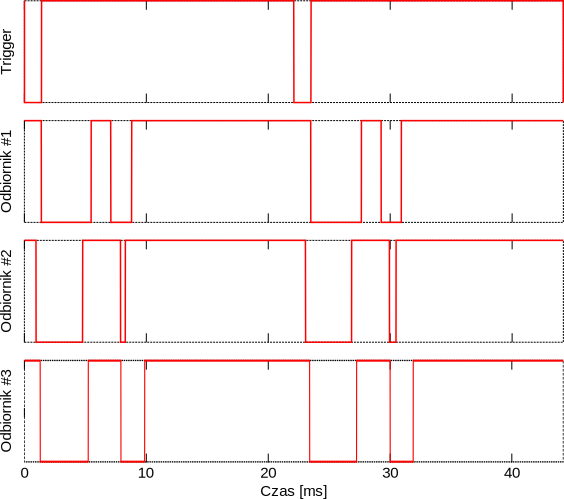
\includegraphics[width=\textwidth]{gfx/odbicia.pdf}
 \caption{Odbicia sygnału dźwiękowego}
 \label{fig:logic_analyzer}
\end{figure}

Porównując długość okresu, w którym nadawany jest sygnał (linia \texttt{Trigger} w stanie niskim) z długością okresu, kiedy odbiornik sygnalizuje odbieranie sygnału (linia odbiornika w stanie niskim), można dostrzec, że nie są one równe. Założyłem, że dźwięk \index{odbicia sygnału}odbił się od pobliskich elementów i dobiegł do odbiornika zanim nastąpił zanik sygnału bezpośredniego.

Na wykresie widać ponadto, że występuje ponowne wygaszenie linii po kilku milisekundach od zakończenia odbierania sygnału. W tym przypadku również zakładałem, że jest to sygnał odbity, który dobiegł do odbiornika.

Dokładniejsze badanie z wykorzystaniem oscyloskopu potwierdzają przypuszczenia. Wyniki tego badania prezentuje rysunek \ref{fig:oscilloscope}\graffito{Sygnał pomiędzy pinem mikrokontrolera, a~punktem testowym jest negowany}.

\begin{figure}
 \includegraphics[width=\textwidth]{gfx/oscyloskop_1.png}
 \caption[Oscylogram sygnału w punkcie testowym]{Oscylogram sygnału w jednym z punktów testowych ukazujący odbicia sygnału}
 \label{fig:oscilloscope}
\end{figure}

\begin{figure}
 \includegraphics[width=\textwidth]{gfx/oscyloskop_attenuated.png}
 \caption{Oscylogram sygnału z dodatkowym tłumieniem}
 \label{fig:oscilloscope_attenuated}
\end{figure}


Aby uwolnić się od wspomnianej usterki, wprowadziłem do kodu mikrokontrolera wymuszone oczekiwanie, którego zadaniem jest upewnienie się, że wszystkie możliwe odbicia sygnału zaniknęły.

Wprawdzie ,,rozwiązanie'' działa, jednak znacząco spowalnia system \ppauza odstęp pomiędzy próbkami wynosi ponad 20ms.

Inną metodą obejścia tego problemu jest zwiększenie tłumienia sygnału rejestrowanego przez odbiornik. Praktyka pokazuje, że takie działanie faktycznie eliminuje problem, z drugiej jednak strony stanowczo pogarsza sprawność systemu, gdyż wymagane jest wtedy znacznie precyzyjniejsze celowanie markerem w odbiorniki. Oscylogram tego badania przedstawia rysunek \ref{fig:oscilloscope_attenuated}.

Z tego też powodu uznałem to za rozwiązanie gorsze, gdyż gracz, który jest docelowym użytkownikiem, w ferworze gry nie może pozwolić sobie na troskanie się sprawnością wykorzystywanego kontrolera.

\textsl{Podsumowanie szybkości działania}
Opierając się na wspomnianych powyżej testach widać, że czynnikiem powodującym największe opóźnienia jest dokładnie ten sam, który najtrudniej wyeliminować, czyli odbicia dźwięku. W związku z wprowadzonymi obejściami problemów, wydajność systemu ograniczona jest do najwyżej 25Hz\graffito{Pełen status nadawany jest co minimum 40ms}.

\paragraph{Porównanie z innymi systemami}
Ze względu na możliwość dostępu do kontrolerów \index{Nintendo!Wiimote}\textsl{Wiimote} oraz \index{Sony!Sixaxis}\textsl{Sixaxis} postanowiłem przeprowadzić porównanie tych urządzeń z moim rozwiązaniem.
\newline

\textsl{Sixaxis}. W celu wyznaczenia prędkości raportowania statusu tego kontrolera wykorzystałem możliwość podłączenia go poprzez port \index{USB}USB oraz obsługę w systemie \index{Linux}Linux w wersji 2.6.35\graffito{Obsługa kontrolera dostępna jest od wersji 2.6.21 z 25.04.2007\citep{Br10}}. Znając wielkość raportu, która wynosi 50 bajtów \citep{Br10}, wystarczy zbadać, jak prędko dane pojawiają się na urządzeniu przyporządkowanym kontrolerowi. 

Należy najpierw zbadać, do jakiego pliku został przyporządkowany do podłączonego urządzenia \ppauza należy w tym celu sprawdzić log kernela za pomocą polecenia \texttt{dmesg}, a następnie zbadać czas, w jakim odczytana zostanie określona z góry ilość danych. Eksperyment ten prezentuje listing~\ref{lst:sixaxis}.

\begin{listing}
  \lstinputlisting{listings/sixaxis.txt}
  \caption{Badanie prędkości kontrolera Sixaxis}
  \label{lst:sixaxis}
\end{listing}

W celu zbadania prędkości pojawiania się danych wykorzystałem program \texttt{dd} z argumentami:
\begin{description}
 \item[\texttt{if=/dev/hidraw4}] określa plik wejściowy, jest on odczytany z wyjścia programu \texttt{dmesg},
 \item[\texttt{of=/dev/null}] określa plik wyjściowy; przekierowując dane do pliku \texttt{/dev/null} upewniam się, że nie wystąpi ograniczenie prędkości operacją zapisu na dysku,
 \item[\texttt{bs=50}] określa rozmiar bloku danych, dzięki temu ustawiony jest bufor będący w stanie przyjąć cały pakiet danych, przez co unikane jest opóźnienie związane z alokacją pamięci,
 \item[\texttt{count=5000}] informuje program o ilości bloków, jakie mają zostać pobrane; ustaliłem dużą wartość w celu wyeliminowania opóźnień, jakie mogłyby wyniknąć w związku z inicjacją i zakończeniem transmisji.
\end{description}

Jak widać, w ciągu prawie dokładnie 50s przetransmitowanych zostało dokładnie 250000 bajtów. Wynika stąd, że prędkość raportowania wynosi
\begin{equation}
 \frac{250000\textrm{b}}{50\textrm{s}} : 50\frac{\textrm{b}}{\textrm{raport}} = 100\textrm{Hz}
\end{equation}

Analizując strukturę raportu, łatwo rozpoznać przyporządkowanie danych do przycisków i policzyć ilość przycisków ,,analogowych''\graffito{Przyciskami analogowymi zwykło nazywać się przyciski, które raportują jak bardzo są naciśnięte}.
\newline

\index{Nintendo!Wiimote}\textsl{Wiimote}. W celu zbadania tego kontrolera wykorzystałem otwartoźródłową bibliotekę \texttt{CWiid}\citep{CWiid}. Zmodyfikowałem źródło jednego z programów, aby raportował czas przyjścia raportu, a następnie w oparciu o informacje o rozmiarach raportów (\citep{Wiibrew}) wybrałem raport, którego rozmiar wynosi dokładnie 18 bajtów, po czym obliczyłem ile raportów przyszło w danym okresie czasu.

Wyniki tego testu pokazuje listing~\ref{lst:wiimote}.

\begin{listing}
  \lstinputlisting{listings/wiimote.txt}
  \caption{Badanie prędkości kontrolera Wiimote}
  \label{lst:wiimote}
\end{listing}

Do pliku \texttt{log} zapisane zostały czasy w formacie \textit{sekundy.nanosekundy}\graffito{W systemach Linux czas reprezentowany jest jako ilość sekund od 1970-01-01T00:00:00Z (ISO 8601)}. W każdej linii pliku zapisana jest dokładnie jedna próbka, dlatego też ilość pobranych próbek wynosi 2500, co pokazuje program \texttt{wc} z argumentem \texttt{-l}. Różnicę pomiędzy rozpoczęciem, a zakończeniem rejestrowania danych prezentuje wynik działania programu \texttt{bc}. Wynika stąd, że prędkość raportowania wynosi
\begin{equation}
 \frac{2500}{25,45\textrm{s}} \approx 100\textrm{Hz}
\end{equation}

Porównanie tych i pozostałych parametrów kontrolerów prezentuje tabela \ref{tab:comparison}.


% http://texblog.net/latex-archive/layout/centering-figure-table/
\begin{table}[b]
  \myfloatalign
\noindent\makebox[\textwidth]{%
\index{Bluetooth} \index{USB} \index{RS232}
\begin{tabularx}{1.5\textwidth}{XXXX} \toprule
    & \emph{Sixaxis} & \emph{Wiimote} & \emph{Nietoperz} \\
    Ilość przycisków & 17 & 11 & 0 \\
    Ilość przycisków ,,analogowych'' & 12 (nie licząc gałek) & 0 & 0 \\
    Komunikacja & Bluetooth, USB & Bluetooth & RS232 \\
    Prędkość raportowania & 100Hz & do 100Hz & poniżej 25Hz \\
    Wielkość raportu statusu & 50 bajtów & do 18 bajtów & 16 bajtów \\
    Możliwość dołączania rozszerzeń & \texttimes & \checkmark & \texttimes \\
    Detekcja ruchów & \index{akceleromter}akcelerometr (3D), \index{żyroskop}żyroskop (1D) & akcelerometr (3D) & ultradźwięki \\
    Dodatkowe funkcjonalności & zdalne uruchamianie konsoli, 4 diody, 2 gałki analogowe & zdalne uruchamianie konsoli, głośnik, kamera IR, 4 diody & 8 diod
  \end{tabularx}}
  \caption{Zestawienie funkcjonalności kontrolerów gier}
  \label{tab:comparison}
\end{table}
%\include{multiToC}
% ********************************************************************
% Backmatter
%*******************************************************
%\appendix
%\cleardoublepage\myPart{Appendix}
%\include{Chapters/Chapter0A}
%********************************************************************
% Other Stuff in the Back
%*******************************************************
\cleardoublepage\include{FrontBackmatter/Bibliography}
\cleardoublepage\include{FrontBackmatter/Colophon}
\cleardoublepage\include{FrontBackmatter/Declaration}
% ********************************************************************
% Game Over: Restart, Restore or Quit?
%*******************************************************
\end{document}
% ********************************************************************
